\section*{Learning Objectives}

By the end of this chapter, students should be able to:
\begin{itemize}
    \item Understand that antidifferentiation is essentially the inverse operation of differentiation.
    \item Comprehend the two Fundamental Theorems of Calculus and explain the precise sense in which differentiation and integration are inverse operations on functions.
    \item Understand that while antidifferentiation and definite integration are technically distinct operations, they are often perceived as identical in the context of Calculus education. This perception is partially justified by their closely related concepts. However, it's crucial to acknowledge the potential drawbacks of this viewpoint, particularly the confusion and discouragement that can arise from the complex rules associated with manually computing antiderivatives.

    \item Appreciate the historical and practical context of computing antiderivatives by hand, and recognize the modern approaches that render hand computations almost obsolete for all but the simplest of cases.
\end{itemize}


\section*{Outcomes}

Upon successful completion of this chapter, students will:
\begin{itemize}
    \item Be introduced to the concept of antiderivatives and familiarize themselves with elementary techniques for finding them.
    \item Gain a thorough understanding of the Fundamental Theorems of Calculus, including their implications in both geometric and analytic contexts.
    \item Develop an insight into the interplay between differentiation, antiderivatives, and definite integration, enhancing their comprehension of calculus as a whole.
    \item Cultivate an appreciation for the traditional methods of finding antiderivatives while also understanding the value and efficiency of using computational tools for real-world applications.
\end{itemize}



\vspace*{2cm}

\renewcommand{\arraystretch}{1.5}  % Adjusts the spacing between rows


\begin{table}[ht!]
\centering
\begin{tabular}{|c|c|c|}
\hline
{\bf Antiderivative \(  \boldint \bm{f(x) \, dx }\)} & {\bf Function \( \bm{f(x)} \) }& {\bf Derivative \( \bm{f'(x)} \) }\\
\hline \hline
\( C \) & \( 0 \) & \( 0 \) \\ \hline
\( kx + C \) & \( k\) & \( 0 \) \\ \hline
\( \frac{1}{3}x^3 + C \) & \( x^2 \) & \( 2x \) \\ \hline
\( e^x + C \) & \( e^x \) & \( e^x \) \\ \hline
\( -\cos(x) + C \) & \( \sin(x) \) & \( \cos(x) \) \\ \hline
\( x\ln(x) - x + C \) & \( \ln(x) \) & \( \frac{1}{x} \) \\ \hline
\( \ln|x| + C \) & \( \frac{1}{x} \) & \( -\frac{1}{x^2} \) \\ \hline
\( -\ln|\cos(x)| + C \) & \( \tan(x) \) & \( 1 + \tan^2(x) \) \\ 
\hline
\end{tabular}
\caption{$C$ is an arbitrary constant, later called a \textbf{constant of integration}. $F(x)$ is an antiderivative of $f(x)$ if $F'(x) = f(x)$. This table illustrates the relationships between an antiderivative, a function, and a derivative. The functions in the middle are the derivatives of the functions in the left column, and the functions in the right column are the derivatives of the functions in the middle column. Going the other direction, the functions in the middle column are antiderivatives of the functions in the right column. As labeled, the functions in the left column are antiderivatives of the functions in the middle column. Bottom line: $F(x) + C$, for $C$ a constant, is always an antiderivative for $f(x):=\frac{dF(x)}{dx}$.}
\label{tab:antideriv-func-deriv}
\end{table}




\section{Introduction} 

This chapter marks a major waypoint in our journey to discover and understand the essence of Calculus. The \textbf{concept of an antiderivative} is a bridge connecting the micro (differential calculus, focused on the infinitesimal, $df$, $dx$, and their ratio) to the macro (integral calculus, focused on adding up an infinite number of vanishingly small areas, $dA = f(x) \, dx$).  As illustrated in Table~\ref{tab:antideriv-func-deriv}, an antiderivative of a function \( f(x) \) is another function \( F(x) \) such that \( F'(x) = f(x) \). The Fundamental Theorems of Calculus elegantly tie together differentiation and integration, showing that these two operations are, in fact, inverse processes. As we unveil the theorems, we will discover the profound connection between the definite integral and antiderivatives, which will further lead us to study indefinite integration and, eventually, improper integrals and differential equations in subsequent chapters.


Because of the Fundamental Theorems of Calculus, the operation of determining antiderivatives shares the same notation as integration, namely
\[ \int f(x) \, dx = F(x) + C, \]
where \( C \) is a \textbf{constant of integration} and $F'(x) = f(x)$. \textcolor{red}{\bf Later, we may regard this elegant formula as the proverbial ``wolf in sheep's clothing''. Intrigued?} 

\bigskip

\begin{tcolorbox}[colback=mylightblue, title = {\bf Antiderivative of a Function}, breakable]

\begin{definition} 
\label{def:antiDerivative}

Let \( f:I \to \real \) be a function defined on an interval \( I \). An \textbf{antiderivative} of \( f \) on the interval \( I \) is a function \( F: I \to \real \) such that
\[
F'(x) = f(x)
\]
for all \( x  \in I \).

\end{definition}

\textbf{Note:} Because $\frac{dC}{dx}=0 $ for all constants $C$, if $F$ is an antiderivative of $f$, then so is $F(x) + C$. In other words, if a function has one antiderivative, it has an infinite number of antiderivatives, and moreover, they all differ by a constant.
\end{tcolorbox}

\bigskip

\begin{example} 
\label{ex:VerifyingAntiderivatives}
In the list of functions (a) - (e) below, identify those functions that are antiderivatives of other functions in the same list.

\begin{enumerate}
\renewcommand{\labelenumi}{(\alph{enumi})}
\setlength{\itemsep}{.2cm}
    \item $f_a(x) = x \cdot \ln(x) - x$
     \item $f_b(x) =  \ln(x) $
      \item $f_c(x) = \ln(x^2)$
       \item $f_d(x) = \cos(x^2)$
        \item $f_e(x) = -2x \cdot \sin(x^2)$
\end{enumerate}
    
\end{example}

\solution This problem is acquainting us with how to check if a given function $F(x)$ is an antiderivative for another function $f(x)$ or not. We apply the definition of what it means to be an antiderivative and check whether $F'(x) = f(x)$ or $F'(x) \neq f(x)$. It is that simple.

\begin{enumerate}
\renewcommand{\labelenumi}{(\alph{enumi})}
\setlength{\itemsep}{.2cm}
    \item $\frac{df_a(x)}{dx} = \ln(x) = f_b(x)$, and hence $f_a(x)$ is an antiderivative of $f_b(x)$. Why? We verify $\left(f_a(x) \right)' = f_b(x)$ by applying the product rule to $x\cdot \ln(x)$ to obtain $\ln(x)+1$. We then differentiate $-x$ to obtain $-1$. Adding up the two derivatives gives us the answer.
     \item $\frac{df_b(x)}{dx} =  \frac{1}{x}$, and hence $f_b(x)$ is NOT an antiderivative of any function in the list. Why? We computed $\left(f_b(x) \right)'$, and it is not equal to any of the functions in the list.
      \item $\frac{df_c(x)}{dx} =  \frac{2}{x}$,  and hence $f_c(x)$ is NOT an antiderivative of any function in the list. 
       \item $\frac{df_d(x)}{dx} = - 2 x \sin\left( x^{2} \right) = f_e(x)$, and hence $f_d(x)$ is an antiderivative of $f_e(x)$.
        \item $\frac{df_e(x)}{dx} =  - 2 \sin\left( x^{2} \right) - 4 x^{2} \cos\left( x^{2} \right)$, and hence $f_e(x)$ is NOT an antiderivative of any function in the list. 
\end{enumerate}

\begin{lstlisting}[language=Julia,style=mystyle]
using Symbolics 

# Create a custom function to make differentiation convenient
function deriv(f, x)
    return expand_derivatives.(Differential(x)(f))
end

# Sample Usage
@variables x # Makes x a symbolic variable
f = x^3*cos(x) + x^2*sin(x)^2 + log(3x) 
dfdx = deriv(f, x)

# Note we do not say f(x) =, just f = 

fa = x * log(x) - x
fb = log(x)
fc = log(x^2)
fd = cos(x^2)
fe = -2x * sin(x^2);
\end{lstlisting}
\textbf{Output} 
\begin{verbatim}
(nothing)
\end{verbatim}

\bigskip

\begin{lstlisting}[language=Julia,style=mystyle]
using Symbolics 

@show dfadx = deriv(fa, x)

@show dfbdx = deriv(fb, x)

@show dfcdx = deriv(fc, x)

@show dfddx = deriv(fd, x)

@show dfedx = deriv(fe, x);
\end{lstlisting}
\textbf{Output} 
\begin{verbatim}
dfadx = deriv(fa, x) = log(x)
dfbdx = deriv(fb, x) = 1 / x
dfcdx = deriv(fc, x) = 2 / x
dfddx = deriv(fd, x) = -2x*sin(x^2)
dfedx = deriv(fe, x) = -2sin(x^2) - 4(x^2)*cos(x^2)
\end{verbatim}

\Qed

\begin{center}
\setlength{\fboxrule}{2pt}  % Setting the thickness of the border line
   \fbox{ \parbox{0.9\linewidth}{
   \vspace{.15cm} 
   
   \textcolor{blue}{\bf How to verify that $\bm{F(x)}$ is an antiderivative of $\bm{f(x)}$? } Simply apply the definition: differentiate $F(x)$ and compare the result to $f(x)$. Hence, given a candidate antiderivative for $f(x)$, verifying or refuting the candidate antiderivative is straightforward. We'll see that finding candidate antiderivatives is, for the most part, anything but straightforward.
}
} 
\end{center}

\bigskip

\begin{example} 
\label{ex:ChatGPTWrongAntiderivatives}

ChatGPT4 (on its own, without an important plugin) has proposed the following antiderivatives for the functions in Example~\ref{ex:VerifyingAntiderivatives}. Determine if they are correct or not.

\begin{enumerate}
\renewcommand{\labelenumi}{(\alph{enumi})}
\setlength{\itemsep}{.2cm} 
\item For \( f_a(x) = x \log(x) - x \):  the antiderivative is \(\int f_a(x) \, dx = \frac{1}{2} x^2 \log(x) - \frac{1}{4} x^2 + C \)

\item For \( f_b(x) = \log(x) \):  the antiderivative is \(\int f_b(x) \, dx = x \log(x) - x + C \)

\item For \( f_c(x) = \log(x^2) \):  the antiderivative is \(\int f_c(x) \, dx = x \log(x^2) - x + C \)

\item For \( f_d(x) = \cos(x^2) \):  the antiderivative is \(\int f_d(x) \, dx = \frac{1}{2} \sqrt{\pi} \text{FresnelS}\left(\sqrt{\frac{2}{\pi}} x\right) + C \)

\item For \( f_e(x) = -2x \sin(x^2) \):  the antiderivative is \(\int f_e(x) \, dx = \cos(x^2) + C \)
\end{enumerate}
\end{example}

\solution ChatGPT4 got two wrong: the antiderivatives for $f_a(x)$ and $f_c(x)$. The antiderivative for $f_d(x)$, \href{https://en.wikipedia.org/wiki/Fresnel_integral}{Wikipedia}, is a special function that we'll talk about later. 

\begin{lstlisting}[language=Julia,style=mystyle]
using Symbolics 

# Proposed by ChatGPT4 31 October 2023, where the 
# constant of integration has been removed
#
AntiDeriv_fa = 0.5 * x^2 * log(x) - 0.25 * x^2
AntiDeriv_fb = x * log(x) - x
AntiDeriv_fc = x * log(x^2) - x
# Function fresnels not readily available in Julia
# AntiDeriv_fd = 0.5 * sqrt(pi) * fresnels(sqrt(2 / pi) * x)
AntiDeriv_fe = cos(x^2)



@show [deriv(AntiDeriv_fa, x) fa]

@show [deriv(AntiDeriv_fb, x) fb]

@show [deriv(AntiDeriv_fc, x) fc]

@show [deriv(AntiDeriv_fe, x) fe];
\end{lstlisting}
\textbf{Output} 
\begin{verbatim}
[deriv(AntiDeriv_fa, x) fa] = Num[x*log(x) x*log(x) - x]
[deriv(AntiDeriv_fb, x) fb] = Num[log(x) log(x)]
[deriv(AntiDeriv_fc, x) fc] = Num[1 + log(x^2) log(x^2)]
[deriv(AntiDeriv_fe, x) fe] = Num[-2x*sin(x^2) -2x*sin(x^2)]
\end{verbatim}

\textcolor{blue}{\bf Missing half of them is not good!} Next, we turn on the Wolfram Plugin and do much better; all of the proposed antiderivatives are correct. Hence, be careful! We did this exercise as a heads-up. Checking the correctness of a proposed antiderivative is typically much easier than finding it. So, just do it!

\begin{lstlisting}[language=Julia,style=mystyle]
# Proposed by ChatGPT4 with the Wolfram Plugin
# 31 October 2024


fa_antiderivative = (1/4) * x^2 * (2 * log(x) - 3)
fb_antiderivative = x * (log(x) - 1)
fc_antiderivative = x * (log(x^2) - 2)
fe_antiderivative = cos(x^2)


@show  [deriv(fa_antiderivative, x) fa]

@show [deriv(fb_antiderivative, x) fb]

@show [deriv(fc_antiderivative, x) fc]

@show [deriv(fe_antiderivative, x) fe];
\end{lstlisting}
\textbf{Output} 
\begin{verbatim}
[deriv(fa_antiderivative, x) fa] = Num[0.5x + 0.5x*(2log(x) - 3) x*log(x) - x]
[deriv(fb_antiderivative, x) fb] = Num[log(x) log(x)]
[deriv(fc_antiderivative, x) fc] = Num[log(x^2) log(x^2)]
[deriv(fe_antiderivative, x) fe] = Num[-2x*sin(x^2) -2x*sin(x^2)]
\end{verbatim}

Simplifying the term ``$0.5x + 0.5x*(2\log(x) - 3)$'' yields ``$x*\log(x) - x$''; all is good! 
\Qed

\bigskip

\begin{funColor}{Pro Tip for Determining Antiderivatives}{ChatGPTforAntiderivatives}

The \texttt{Symbolics.jl} package can compute simple antiderivatives. The competing package, \texttt{SymPy.jl}, is somewhat better. However, the hands-down winners are the tools from Wolfram, namely \href{https://www.wolfram.com/mathematica/}{Mathematica} and the \href{https://www.wolfram.com/wolfram-plugin-chatgpt/}{Plugin} for ChatGPT, and the tools from \href{https://www.maplesoft.com/products/Maple/}{MapleSoft}. Of these, the easiest to use is ChatGPT with the Wolfram plugin. Below is the prompt that generated the correct antiderivatives for Example~\ref{ex:ChatGPTWrongAntiderivatives}.

\begin{verbatim}
Can you provide antiderivatives for the following functions using the Wolfram plugin?
fa = x * log(x) - x
fb = log(x)
fc = log(x^2)
fd = cos(x^2)
fe = -2x * sin(x^2);

I'd like the answers in two separate forms:
1) All answers in latex
2) All answers in a form that Julia can use. 
\end{verbatim}

Sure! Here are the antiderivatives for the given functions:

1) In LaTeX:
\begin{itemize}
    \item  \( \int (x \log(x) - x) \, dx = \frac{1}{4} x^2 (2 \log(x) - 3) + C \)
   \item \( \int \log(x) \, dx = x (\log(x) - 1) + C \)
   \item \( \int \log(x^2) \, dx = x (\log(x^2) - 2) + C \)
   \item \( \int \cos(x^2) \, dx = \sqrt{\frac{\pi}{2}} C_F\left(\sqrt{\frac{2}{\pi}} x\right) + C \) (where \( C_F \) is the Fresnel C integral)
   \item \( \int (-2x \sin(x^2)) \, dx = \cos(x^2) + C \)
\end{itemize}
and \( C \) is the constant of integration.\\

2) In a form that Julia can use:
\begin{verbatim}
   - `fa_antiderivative(x) = (1/4) * x^2 * (2 * log(x) - 3)`
   - `fb_antiderivative(x) = x * (log(x) - 1)`
   - `fc_antiderivative(x) = x * (log(x^2) - 2)`
   - `fd_antiderivative(x) = sqrt(pi/2) * fresnelc(sqrt(2/pi) * x)` 
            (Note: Julia has a `fresnelc` function in the `SpecialFunctions` package)
   - `fe_antiderivative(x) = cos(x^2)`
\end{verbatim}
  
\end{funColor}

\bigskip

% \begin{example} Compute the antiderivtive for 
% $$ f(x):=
% \frac{2  x^{3 } \cos\left( x \right) \sin\left( x \right) e^{2  + \sin^{2 }\left( x \right)}}{1  + \left( e^{2  + \sin^{2 }\left( x \right)} \right)^{2 }} + 3  x^{2 } \arctan\left( e^{2  + \sin^{2 }\left( x \right)} \right).
% $$    
% \end{example}

% \solution Using ChatGPT and the Wolfram plugin, the answer is 
% \[ x^3 \arctan\left(e^{\frac{1}{2} (5 - \cos(2x))}\right) + \text{C}. \]
% Moreover, the answer is correct, because the problem was created by differentiating $F(x):= x^3  \cdot \atan(\exp(\sin(x)^2 + 2)) \cdot \log(x^2 + 1) $ with respect to $x$. The trig identity,  \( \sin^2(x) = \frac{1 - \cos(2x)}{2} \), allows one to show that $\sin(x)^2 + 2 = \frac{(5 - \cos(2x))}{2}$. While few humans would want to take on this ``integration problem'' using the tools taught in Calc II, software tools can take it on. 

% \Qed

% \bigskip

\begin{example} Compute the antiderivtive for 
$$ f(x):=
\frac{2  x^{3 } \cos\left( x \right) \sin\left( x \right) e^{2  + \sin^{2 }\left( x \right)}}{1  + \left( e^{2  + \sin^{2 }\left( x \right)} \right)^{2 }} + 3  x^{2 } \arctan\left( e^{2  + \sin^{2 }\left( x \right)} \right).
$$    
\end{example}

\solution Using ChatGPT and the Wolfram plugin, the answer is 
\[ x^3 \arctan\left(e^{\frac{1}{2} (5 - \cos(2x))}\right) + \text{C}. \]
Moreover, the answer is correct because the problem was created by differentiating $F(x):= x^3  \cdot \atan(\exp(\sin(x)^2 + 2)) \cdot \log(x^2 + 1) $ with respect to $x$. The trig identity,  \( \sin^2(x) = \frac{1 - \cos(2x)}{2} \), allows one to show that $\sin(x)^2 + 2 = \frac{(5 - \cos(2x))}{2}$. Few humans would want to take on this ``integration problem'' using the tools taught in Calc II. \textcolor{blue}{\bf What ChatGPT accomplished with the Wolfram plugin is impressive.}

\Qed

\bigskip

\begin{example}  Compute the antiderivtive for 
    \begin{equation}
    \begin{aligned}
        f(x) &= 3  x^{2 } \sqrt{2  + \left( \log\left( 1  + x^{2 } \right) \right)^{2 }} \arcsin\left( e^{2  + \sin^{2 }\left( x \right)} \right) \\[1em]
        & + \frac{2  x^{4 } \log\left( 1  + x^{2 } \right) \arcsin\left( e^{2  + \sin^{2 }\left( x \right)} \right)}{\sqrt{2  + \left( \log\left( 1  + x^{2 } \right) \right)^{2 }} \left( 1  + x^{2 } \right)} \\[1em]
        & + \frac{2  x^{3 } \cos\left( x \right) \sin\left( x \right) e^{2  + \sin^{2 }\left( x \right)} \sqrt{2  + \left( \log\left( 1  + x^{2 } \right) \right)^{2 }}}{\sqrt{1  - \left( e^{2  + \sin^{2 }\left( x \right)} \right)^{2 }}}.
    \end{aligned}
\end{equation}
\end{example}

\solution \textcolor{red}{\bf WolframAlpha query was not successful or did not return the expected format.} Nevertheless, 

\begin{equation}
f(x) =  \frac{ d}{dx} \underbrace{\left(  x^{3} \cdot \arcsin\left( e^{2.0 + \sin^{2}\left( x \right)} \right) \cdot \sqrt{2 + \left( \log\left( 1 + x^{2} \right) \right)^{2}} \right)}_{F(x)},
\end{equation}
and hence, a ``relatively simple'' antiderivative $F(x)$ exists, despite the Wolfram Plugin failing to find it. The full \href{https://www.wolfram.com/mathematica/}{Mathematica} or \href{https://www.maplesoft.com/products/Maple/}{MapleSoft} desktop tools would likely be able to solve the problem.
\Qed




\section{Uniting Integration and Differentiation through the Fundamental Theorems of Calculus}

The \textbf{First Fundamental Theorem of Calculus} states that every continuous function has an antiderivative. The \textbf{Second Fundamental Theorem of Calculus} states that all definite integrals can be evaluated through antiderivatives. Together, these two results seamlessly tie together integration and differentiation as ``inverse operations''. 

\subsection{Fundamental Theorems}

\begin{propColor}{Fundamental Theorems of Calculus}{FundamentalTheoremsCalculus}

\textbf{First Fundamental Theorem of Calculus:}
Let \( f:[a, b] \to \real \) be a continuous real-valued function defined on a closed interval \([a, b]\). Then, the function \( F:[a, b] \to \real \) defined by
\begin{equation}
    \label{eq:FirstFundThmCalculusVo1}
F(x) = \int_a^x f(t) \, dt
\end{equation}
for all \( x \in [a, b]\), is continuous on \([a, b]\), differentiable on the open interval \( (a, b) \), and \( F'(x) = f(x) \) for all \( x \in  (a, b) \). You will also see it written as 
\begin{equation}
    \label{eq:FirstFundThmCalculusVo2}
   \frac{d}{dx}  F(x) =  \frac{d}{dx} \left[ \int_a^x f(t) \, dt \right] = f(x),
\end{equation}
to emphasize that differentiation undoes, or inverses, integration.
\\

\textbf{Second Fundamental Theorem of Calculus:}
Let \( f:[a, b] \to \real \) be a real-valued function defined on a closed interval \([a, b]\) that admits an antiderivative \( F \) on \([a, b]\), that is, $F:[a, b] \to \real$ is differentiable on $(a, b)$ and for all $x \in (a, b)$, $F'(x) = f(x)$. Then,  \( f \) is integrable on \([a, b]\) and
\begin{equation}
    \label{eq:SecondFundThmCalculusVo1}
\int_a^b f(x) \, dx = F(x) \Big|_a^b := F(b) - F(a).
\end{equation}
You will also see it written as 
\begin{equation}
    \label{eq:SecondFundThmCalculusVo2}
\int_a^b \frac{dF(x)}{dx} \, dx = F(x) \Big|_a^b := F(b) - F(a), 
\end{equation}
to underline that integration undoes, or inverses, differentiation.

\bigskip

\textbf{Notes:} For a nuanced presentation of the First Fundamental Theorem of Calculus, we recommend \href{https://youtu.be/tgOgjbYs97A}{3 Levels of Proving the Fundamental Theorem of Calculus} by Trivial. The first part of the video \href{https://youtu.be/Jk_k3q9RoMU?t=127}{The Essence of (Multivariable) Calculus} by Foolish Chemist provides an intuitive treatment of the Second Fundamental Theorem of Calculus. If you exceed the 6:20 mark, you'll be into multivariable versions of the Fundamental Theorems. Yikes! 
\end{propColor}


\subsection{Using the Second Fundamental Theorem of Calculus for Definite Integration}

    Let's roll up our sleeves and get to work using the Second Fundamental Theorem of Calculus to evaluate some definite integrals. It looks super easy, right? In Table~\ref{tab:CommonFunctionsAndTheirDerivatives} we had a list of functions and their derivatives. Based on the First Fundamental Theorem of Calculus, we can repurpose our table to give us a list of antiderivatives, like so,

    \bigskip

\renewcommand{\arraystretch}{1.5}
\begin{table}[htb]
\centering
\begin{tabular}{|c |c|c|c|c|c|c|c|c|c  |}
\hline
{\bf Function} & $C$ & $\frac{x^{k+1}}{k+1}+C $ & $e^x +C$ & $\ln|x| +C$ & $\sin(x)+C$ & $\cos(x)+C$ & $\tan(x)+C$ & $\atan(x)+C$ & {\bf Antiderivative}\\
\hline
{\bf Derivative} & $0$ & $x^k$ & $e^x$ & $\frac{1}{x}$ & $\cos(x)$ & $-\sin(x)$ & $1 + \tan^2(x)$ & $\frac{1}{1 + x^2}$ & {\bf Function}\\
\hline
\end{tabular}
\caption{Common Elementary Functions and their Antiderivatives (Worth committing to memory to showcase your expertise). When doing antiderivatives, it is more convenient to have the monomials presented as given here than how we did the monomial entry in Table~\ref{tab:CommonFunctionsAndTheirDerivatives}. In addition, we've extended the natural logarithm to negative numbers via an absolute value. Otherwise, the two tables are the same.}
\label{tab:CommonFunctionsAndTheirAntiderivatives}
\end{table}

\bigskip 
\emstat{
\textbf{Why is there an absolute value on the natural logarithm?} Note that $\frac{1}{x}$ is defined for all $x \neq 0$. Hence, its domain can be $(0, \infty)$, the positive reals, or  $(-\infty, 0)$, the negative reals. Logarithms, on the other hand, are only defined for the positive reals. When $x>0$, $|x|=x$, and hence, $ \frac{d}{dx} \ln|x| = \frac{d}{dx} \ln(x) = \frac{1}{x}$. When $x < 0$, $|x| = -x$, and then, by the Chain Rule,
$$\frac{d}{dx} \ln|x| = \frac{d}{dx} \ln(-x) = \frac{1}{-x} \cdot (-1) = \frac{1}{x},$$
where the $(-1)$ comes from differentiating $-x$ with respect to $x$. While it is never wrong to include the absolute value sign in the antiderivative of $\frac{1}{x}$, when the context makes it clear that $x >0$, it is standard practice to drop it because, then, $|x|=x$.\\

You can also think about the derivative of the natural logarithm as follows. From the Chain Rule, Chain Rule, $\frac{d}{dx} \ln(g(x)) = \frac{1}{g(x)} \cdot \frac{dg(x)}{dx}$, for $g(x) > 0.$ Substituting in $g(x) = |x|$ and $x\neq 0$, yields, 
$\frac{d}{dx} \ln(|x|) = \frac{1}{|x|} \cdot \frac{d}{dx} |x|.$
When $x>0$,  $\frac{d}{dx} |x| = 1$ and when $x<0$,  $\frac{d}{dx} |x| = -1$. Hence, 
$$  \frac{1}{|x|} \cdot \frac{d}{dx} |x| = \begin{cases}
    \frac{1}{x} \cdot 1 & x > 0 \\
    \frac{1}{-x} \cdot (- 1)  & x < 0
\end{cases}~~ = \frac{1}{x}~~ \text{for}~~ x \neq 0.$$
}

\bigskip

\begin{example} On the basis of Table~\ref{tab:CommonFunctionsAndTheirAntiderivatives} and the Fundamental Theorems of Calculus, compute the following definite integrals.
\begin{enumerate}
\renewcommand{\labelenumi}{(\alph{enumi})}
\setlength{\itemsep}{.2cm}
    \item $\int_1^5 \left(2 x^3 + e^x \right)\,dx$
     \item  $\int_1^e \left(\frac{1}{x}+ \frac{1}{1 + x^2} \right)\,dx$
       \item $\int_0^\pi \left( \sin(x) + 3 \cos(x) \right)\,dx$
        \item $\int_0^1 \left(  \frac{x}{1 + x^2}\right)\,dx$
\end{enumerate}
    
\end{example}

\solution


\begin{enumerate}
\renewcommand{\labelenumi}{(\alph{enumi})}
\setlength{\itemsep}{.2cm}
    \item The antiderivative of $x^3$ is $\frac{x^4}{4}$ and the antiderivative of $e^x$ is itself, $e^x$. Hence, 
    $$\int_1^5 \left(2 x^3 + e^x \right)\,dx =    \underbrace{\left(2 \cdot \frac{x^4}{4} + e^x \right)}_{\text{antideriv.}~F(x)} \underbrace{\Bigg|_{a=1}^{b=5}}_{\text{limits}} =  \underbrace{\left( \frac{5^4}{2} + e^5\right)}_{F(b)}  - \underbrace{\left( \frac{1^4}{2} + e^1\right)}_{F(a)} = 312 + e^5 - e \approx 457.69.$$
    
     \item  The antiderivative of $\frac{1}{x}$ is $\ln(x)$ and the antiderivative of $\frac{1}{1 + x^2}$ is $\atan(x)$. Hence, 
    \begin{align*}
        \int_1^e \left(\frac{1}{x}+ \frac{1}{1 + x^2} \right)\,dx &=    \underbrace{\left( \ln(x) +  \atan(x) \right)}_{\text{antideriv.}~F(x)} \underbrace{\Bigg|_{a=1}^{b=e}}_{\text{limits}} \\
        &=  \underbrace{\left( \ln(e) +  \atan(e)\right)}_{F(b)}  - \underbrace{\left( \ln(1) +  \atan(1)\right)}_{F(a)} = 1 + \atan(e) - \atan(1) \approx 1.43.
    \end{align*}    
     
   
      \item The antiderivative of $\sin(x)$ is $-\cos(x)$ and the antiderivative of $\cos(x)$ is $\sin(x)$. Hence, 
    \begin{align*}\int_0^\pi \left( \sin(x) + 3 \cos(x)\right)\,dx &= \left( -\cos(x) + 3\sin(x)\right) \Bigg|_0^\pi =    \underbrace{\left(-\cos(x) + 3\sin(x) \right)}_{\text{antideriv.}~F(x)} \underbrace{\Bigg|_{a=0}^{b=\pi}}_{\text{limits}} \\
    &=  \underbrace{\left( -\cos(\pi) + 3\sin(\pi)\right)}_{F(b)}  - \underbrace{\left( -\cos(0) + 3\sin(0)\right)}_{F(a)} = 2.
    \end{align*}


        \item The antiderivative of $ \frac{x}{1 + x^2}$ is NOT in Table~\ref{tab:CommonFunctionsAndTheirAntiderivatives}. Hence, we either have to compute it via ChatGPT+Wolfram or learn a more powerful means for generating antiderivatives. From ChatGPT+Wolfram, we have the antiderivative of $\frac{x}{1 + x^2}$ is $0.5 \log(x^2 + 1)$. Hence, 
        
        $$\int_0^1 \left(  \frac{x}{1 + x^2}\right)\,dx = 0.5 \log(x^2 + 1) \Bigg|_0^1 = 0.5 \log(2) - 0.5\log(1) = 0.5 \log(2) \approx 0.34657$$
\end{enumerate}

\bigskip
\begin{lstlisting}[language=Julia,style=mystyle]
# Our prior means of computing definite integrals as a double check
using QuadGK
ansA,  = quadgk(x ->2x^3 + exp(x), 1, 5)
ansB,  = quadgk(x ->(1/x) + (1/(1+x^2)), 1, exp(1))
ansC,  = quadgk(x ->sin(x) + 3cos(x), 0, pi)
ansD,  = quadgk(x ->x/(1+x^2), 0, 1);
[ansA, ansB, ansC, ansD]
\end{lstlisting}
\textbf{Output} 
\begin{verbatim}
4-element Vector{Float64}:
 457.69487727411763
   1.4328847416198296
   2.000000000000001
   0.3465735902799727
\end{verbatim}

\Qed

\bigskip

\emstat{ \textbf{Taking Stock:} For simple, ``everyday'' functions, it is relatively easy to use the Second Fundamental Theorem of Calculus for evaluating definite integrals. It can be a bit tedious because we have to find the antiderivative for each term in the integral, and then we have to evaluate the antiderivatives at the limits of integration, but conceptually, it is straightforward. Obtaining the antiderivatives is clearly the most difficult part of this process. For some super common functions, we have the antiderivatives available in a standard table, or even memorized. For less common functions, we have to determine the antiderivatives ourselves, one way or another. In Julia, the process of determining the antiderivatives and plugging in values is certainly harder than just running \texttt{quadgk} on the original functions. \textcolor{red}{\bf So, when should we compute antiderivatives to evaluate integrals?} \\

\begin{itemize}
\item When you seek to establish a general result about an integral, having the closed-form solution provided by an antiderivative is highly useful. What is the volume of a sphere of radius $r>0$? Quadgk can only compute the result for a specific value of $r$, and not for $r>0$ a variable.
    \item In real-time coding for robotics, your available computing resources may be too slow to run \texttt{quadgk} over and over. Being able to compute the answer to an integral in closed form may provide for ultra-fast function evaluation. In this case, knowledge (i.e., Fundamental Theorems of Calculus) is power!
    \item {\bf When you do not have Julia handy, such as in an exam.} 
    \item When a HW problem in an engineering course asks you to integrate a function and show your work, 99.9\% of the time, you are expected to use antiderivatives and the Fundamental Theorems of Calculus because that is what the instructors and teaching assistants learned. It will take time for the Education Community to accept numerical computation in the classroom. In engineering practice, don't worry. Industry is all over this. 
    \item When you want to enter an \href{https://www.youtube.com/results?search_query=integration+bees}{Integration Bee}. Just like a \href{https://www.youtube.com/results?search_query=spelling+bees}{Spelling Bee}, it takes a lot of practice and rote memorization. Just as being a Spelling Bee Champ does not put you on the road to becoming a creative writer, being an Antiderivative Champ does not put you on the road to becoming a creative engineer or mathematician. 
\end{itemize}
}

\subsection{Conflating Integration and Antiderivatives is a Pedagogical Pitfall in Calculus}
\label{sec:PedagogicalPitfall}

In this book, we have endeavored to maintain a clear distinction between definite integrals and integration via antiderivatives. For starters, we treat them in separate chapters. However, in broader discourse (aka, the big-bad world outside the course), the distinction might not always be as clear-cut, and the sense of the action verb `` to integrate'' must be extracted from the surrounding context. The notation of calculus, while often elegant and succinct, is not helpful in this regard. 

In the context of definite integrals, the integral sign  \(\int\) is accompanied by limits of integration, as in \(\int_a^b f(x) \, dx\), indicating the interval over which the function \(f\) is to be integrated. However, when we venture into the domain of antiderivatives or indefinite integrals, the integral sign stands alone, 
\[ \int f(x) \, dx,\] 
and represents a family of functions whose derivative is \(f\). An alternative notation for denoting antiderivatives, albeit less common, is to use the differentiation symbol with a negative exponent, as in 
\[ D^{-1}f ~~~\text{  or  } ~~~\frac{d^{-1}}{dx^{-1}} f(x). \] 
This notation explicitly mirrors the inverse operation being performed relative to differentiation. Yet, it's not widely adopted, perhaps due to its unwieldiness or the potential confusion with reciprocal functions. Because the notation has yet to ``go viral'' ---three hundred years and waiting---we do not use it.

The transition from \(\int_a^b f(x) \, dx\) to \(\int f(x) \, dx\) marks the evolution from a concrete computation to a more abstract concept, mirroring the increase in abstraction from arithmetic to algebra. On one hand, antidifferentiation does amplify the power of Calculus. On the other hand, all too often, the numerous methods for computing antiderivatives become the ``be all and end all'' of a standard Calc II course, leading many students to throw up their hands and walk away. 

How could that be? As we'll explain in the next Section, the methods for computing antiderivatives are based on inverting the differentiation rules in Prop.~\ref{thm:DifferentiationRules}. Becoming proficient in them takes a lot of effort and is typically accompanied by deep frustration on the part of the learner. The frustration arises because (a) knowing when to use one method over another requires significant experience; (b) each method typically involves multiple steps where a simple minus sign error or confusing a multiply by a constant with a divide by the same constant destroys the entire calculation, and finally, (c), once you have computed the antiderivative, beyond the satisfaction of having solved a cool puzzle, you rarely get to use it for \href{https://youtu.be/69xFhaUFKk0}{something meaningful}. In real engineering, you are unlikely to use the hand methods of computing antiderivatives with sufficient frequency to maintain fluency, supposing you master them while in College.  \\

You were once taught how to extract a square root by hand. How often do you do that now? \textcolor{blue}{\bf This textbook takes the attitude that while there was a time when it made sense to learn how to execute by hand all of the methods for computing antiderivatives, that time has passed.} Yes, it's almost always true that ``knowledge is power''. Understanding the concepts underlying the ``hand methods of integration'' is sometimes useful. In Linear algebra, however, once we understood the basic workings of a determinant or the LU Factorization, we were happy to turn the actual computations over to an algorithm; the same is true of the rules for computing antiderivatives and definite integrals: we want an algorithm. \\

\textcolor{blue}{\bf The next section will work through enough methods and examples so that when you are required to compute antiderivatives by hand in an engineering course, you are prepared.} 

\section{The Art of the Antiderivative: Inverting Differentiation Rules to Find Antiderivatives}

We go through, roughly in order of importance, various strategies for finding antiderivatives of functions. 

\subsection{The Power Rule of Integration: Inverts the Power Rule of Differentiation}

From the power rule for differentiation, we have that $\frac{d}{dx} x^{k+1} = (k+1)x^{k}$. Hence, by the Second Fundamental Theorem of Calculus,
\begin{equation}
    \label{eq:PowerRuleIntegration}
    \int x^{k}\, dx = \frac{x^{k+1}}{k+1} + C.
\end{equation}

\bigskip

\begin{example}
Compute an antiderivative for  $4 x^2$.
\end{example}
\solution By the Power Rule, $ \int 4 x^2 \, dx = 4 \left( \frac{x^3}{3} + C_1 \right) =  \frac{4}{3} \, x^3 + C$, where $C:=4 C_1$.
\Qed

\bigskip


\subsection{The Fundamental Rule: Integrating the Differential}
\textcolor{blue}{\bf When doing an integral by hand that is harder than a monomial, our first thought should be: can we recognize the integrand (aka, the function being integrated) as being the derivative of a commonly known function}. The most fundamental relationship between differentiation and integration is given by the total differential of a function, 
\[ df(x) = \frac{df(x)}{dx} \, dx = f'(x)\, dx. \]
The Second Fundamental Theorem of Calculus says that integrating both sides with respect to \( x \) gives us back the original function (up to a constant of integration):
\begin{equation}
\label{eq:FundamentalRule4Integration}
    \int df(x) = \int \frac{df(x)}{dx} \, dx = \int f'(x) \, dx =f(x) + C.
\end{equation} 

\bigskip

\begin{example}
Compute an antiderivative for  $3x^2$.
\end{example}
\solution Here, we recognize that \( x^2 = \frac{d}{dx}\left( \frac{x^3}{3} \right) = \left( \frac{x^3}{3} \right)'\). Therefore, the Second Fundamental Theorem of Calculus gives us
\[ \int 3x^2 \, dx = \int 3 \left( \frac{x^3}{3} \right)' \, dx = 3 \frac{x^3}{3} + C = x^3 + C. \]
\Qed

\bigskip

\begin{example}
Determine \( \int 13\, ( 1 + \tan^2(x)) \, dx \). 
\end{example}
\solution This is an antiderivative problem. From Table~\ref{tab:CommonFunctionsAndTheirAntiderivatives}, we recognize that \(  1 + \tan^2(x) = \frac{d}{dx}\left( \tan(x) \right) = \left(\tan(x) \right)'\). Therefore, the Second Fundamental Theorem of Calculus gives us
\[ \int 13\, ( 1 + \tan^2(x))  \, dx = \int 13 \left(\tan(x) \right)' \, dx = 13 \tan(x) + C. \]
\Qed

\bigskip

Admittedly, these are not impressive integrals, but as the saying goes, \href{https://www.merriam-webster.com/dictionary/look%20a%20gift%20horse%20in%20the%20mouth}{do not look a gift horse in the mouth}.

\subsection{Inverting the Chain Rule: Integration by Substitution, aka u-Substitution}

The chain rule for differentiation states that if \( f'(x) = \frac{df(x)}{dx} \) and  \( g'(x) = \frac{dg(x)}{dx} \) exist, then 
$$ \frac{d}{dx} \left(f(g(x)) \right)= \left( f(g(x))\right)' = f'(g(x)) \cdot g'(x).$$
To invert this, we use \textbf{integration by substitution}. If we define $u=g(x)$, then $du = \frac{dg(x)}{dx}\, dx = g'(x)\, dx $, and 
\begin{equation}
    \int \underbrace{f'(g(x))}_{f'(u)} \cdot \underbrace{g'(x) \, dx}_{du} = \int f'(u)\, du = f(u) + C =  f(g(x)) + C, 
\end{equation}
after substituting in $u=g(x)$. In other words, by a clever substitution, we turn something that did not look like a total differential into something that is a recognizable total differential so that the Fundamental Rule in \eqref{eq:FundamentalRule4Integration} can be applied. Yeah, computing $\int f'(u)\, du$ is easy, while $\int f'(g(x)) \cdot g'(x) \, dx$ looks hard before making the substitution. This is an example of useful pattern matching: looking for instances of the chain rule appearing as the integrand (aka, under the integral sign).


\bigskip 
\begin{rem} (\textbf{u-Substitutions}) 
    It is common practice to use $u(x)$ instead of $g(x)$ AND to call this the Method of $u$-Substitution. Why $u$? When you find a satisfying answer, let us all know.
\end{rem}

\bigskip

\begin{example} 
\label{ex:uSubstiutionExamp01}
Use integration to find \( \int 3x \cos(x^2 + 1) \, dx \).
\end{example}

\solution  Integrate, here, means to find an antiderivative. Table~\ref{tab:CommonFunctionsAndTheirAntiderivatives} does not contain an antiderivative for $3x \cos(x^2 + 1)$. However, we see that the cosine function has been composed with $x^2 + 1$, and lucky for us, its derivative, $2x$, is ALMOST sitting in front of the function. Inspired by this, we let $f'(x) = \cos(x)$ and \( u(x) = x^2 + 1 \) so that \( du = 2x \, dx \). Then,
\[ \int 3x \cos(x^2 + 1) \, dx = \frac{3}{2} \cdot  \int 2x \cos(x^2 + 1) \, dx =\frac{3}{2} \cdot\int \cos(u) \, du = \frac{3}{2} \cdot\sin(u) + C = \frac{3}{2} \cdot \sin(x^2 + 1) + C, \]
after substituting in $u = x^2 + 1$.
\Qed

\bigskip

\begin{example} 
\label{ex:uSubstiutionExamp02}
Compute the definite integral \( \int_0^\pi 2x \cos(x^2 + 1) \, dx \). 
\end{example}

\solution We give two solutions, one that obliges us to complete the last step of substituting $u = u(x)$ back into $f(u)$ and one that allows us to avoid that step. \\

\textbf{Approach One:} From example~\ref{ex:uSubstiutionExamp01}, we know the antiderivative of $2x \cos(x^2 + 1)$ is $F(x):=f(u(x)) = \sin(x^2 + 1) + C$. By the Second Fundamental Theorem of Calculus,
$$
\int_0^\pi 2x \cos(x^2 + 1) \, dx = F(\pi) - F(0) = \left(\sin(\pi^2 + 1) + C \right) - \left( \sin(0^2 + 1) + C \right) = \sin(\pi^2 + 1) - \sin(1).
$$
\textcolor{blue}{\bf Because the constant of integration $C$ always cancels out, it is common not even to write it down when using antiderivatives for definite integrals.}

\textbf{Approach Two:} The limits of integration $a=0$ and $b=\pi$ really mean the $x$-lower limit of integration is $0$ and the $x$-upper limit of integration is $\pi$, When we perform a change of variables $u(x)$, we can also change the limits of integration to present the $u$-lower limit of integration and the $u$-upper limit of integration, which are $u(a) = u(0) = \sin(1)$ and $u(b) = u(\pi) = \sin(\pi^2 + 1)$. Hence, we'd compute the integral as 
$$
\int_0^\pi 2x \cos(x^2 + 1) \, dx =  \int_{u(0)}^{u(\pi)} \cos(u)\, du = \sin(u) \Bigg|_{1}^{\pi^2 + 1} =  \sin(\pi^2 + 1) - \sin(1).
$$
When the antiderivative is more complicated, the second approach becomes more valuable. In addition, when the first substitution only gets you halfway there, and a second substitution is required, this second approach really shines. It's also common to add extra notation to help one keep track of the limits carefully when doing a change of variable, such as 
$$
\int_{x=0}^{x = \pi} 2x \cos(x^2 + 1) \, dx =  \int_{u = u(0)}^{u = u(\pi)} \cos(u)\, du = \sin(u) \Bigg|_{u = 1}^{u = \pi^2 + 1} =  \sin(\pi^2 + 1) - \sin(1);
$$
\textcolor{blue}{\bf this helps avoid a really bad error}, where the original limits are carried forward as in 
$$
\int_{0}^{\pi} 2x \cos(x^2 + 1) \, dx ~~{\RED =} \int\limits_{\textcolor{red}{0}}^{\textcolor{red}{\pi}} \cos(u)\, du = ~\RED  \sin(u) \Bigg|_{0}^{\pi} = ~\sin(\pi) - \sin(0) = 0,
$$
and everything in red is wrong!
\Qed



\bigskip

\begin{example} 
\label{ex:uSubstiutionExamp04}
Suppose that $f(x)$ is the antiderivative of $f'(x)$. Find the antiderivative of $f'(\alpha x - x_0)$, where $\alpha \neq 0$  and $x_0 \in \real$ are constants.
\end{example}
\solution We define $u(x):=\alpha x - x_0 $ and note that $f'(u(x)) = f'(\alpha x - x_0)$. Moreover, $du(x) = \alpha\, dx \implies dx = \frac{1}{\alpha} \, du$. Hence, 
\begin{equation}
    \int f'(\alpha x - x_0)\, dx = \int f'(u)\, \frac{1}{\alpha}\, du =\frac{1}{\alpha} f(u) + C = \frac{1}{\alpha} f(\alpha x - x_0) + C.
\end{equation}
\Qed

\textcolor{blue}{\bf Using the above result, we can immediately expand our table of known antiderivatives to include scaling and shifting. }

 %  \alpha x  - x_0   (\alpha x - x_0)

%    \frac{1}{\alpha}

\renewcommand{\arraystretch}{1.8}
\begin{table}[htb]
\centering
{\small % Reduce the font size
\setlength\tabcolsep{3pt} % Reduce the space between columns
\begin{tabular}{|c |c|c|c|c|c|c|c|}
\hline
{\bf Antiderivative} & $\frac{1}{\alpha} \frac{(\alpha x - x_0)^{k+1}}{k+1} $ & $\frac{1}{\alpha} e^{ (\alpha x - x_0)} $ & $\frac{1}{\alpha} \ln|\alpha x - x_0|$ & $\frac{1}{\alpha} \sin(\alpha x  - x_0 )$ & $\frac{1}{\alpha} \cos(\alpha x  - x_0 )$ & $\frac{1}{\alpha} \tan(\alpha x  - x_0 )$ & $\frac{1}{\alpha}\atan(\alpha x  - x_0 )$ \\
\hline
{\bf Function} &  $(\alpha x - x_0)^k$ & $e^{ (\alpha  x- x_0)}$ & $\frac{1}{(\alpha x - x_0)}$ & $\cos(\alpha x  - x_0 )$ & $-\sin(\alpha x  - x_0 )$ & $1 + \tan^2(\alpha x  - x_0 )$ & $\frac{1}{1 + (\alpha x  - x_0 )^2}$ \\
\hline
\end{tabular}
}
\caption{Common Elementary Functions and their Antiderivatives. The constants of integration, $C$, have been dropped to save space.}
\label{tab:CommonFunctionsAndTheirAntiderivativesWithScalingShift}
\end{table}


\bigskip

\begin{example} 
\label{ex:uSubstiutionExamp03}
Compute the indefinite integral \( \int \frac{\left( \ln|x|) \right)^2}{x} \, dx \). 
\end{example}

\solution \Ans \( \int \frac{\left( \ln|x| \right)^2}{x} \, dx = \frac{\left(\ln(x) \right)^3}{3} + C\) for any domain $[a, b]$ that excludes $x=0$.


The problem is using different vocabulary for the antiderivative so that we get used to the idea that for most students of Calculus, integration and antidifferentiation are one and the same, two peas in the same pod, identical twins; you get the picture. Once again, we cannot find the integrand in Table~\ref{tab:CommonFunctionsAndTheirAntiderivatives}. If we take $f'(x) = x^2$ and $u(x) = \ln|x|$, then $u'(x) = \frac{1}{x}$ and $du = \frac{1}{x} \, dx$. Hence, we have that 
$$ \frac{\left( \ln|x| \right)^2}{x} \, dx = u^2 \, du = f'(u) \, du$$
Because we know that the antiderivative of $f'(u)=u^2$ is $f(u)= \frac{u^3}{3}$, we have
$$ \int \frac{\left( \ln|x| \right)^2}{x} \, dx = \int u^2 \, du = \frac{u^3}{3} + C= \frac{\left(\ln|x| \right)^3}{3} + C.$$

\Qed

\bigskip

\begin{funColor}{``Danger, Will Robinson!'' is 1960's Slang for ``Red Flag!''}{RobotSlang}

\begin{center}
    {\Large Because \textcolor{blue}{\bf Danger, Will Robinson!} is tied to a robot, we use it in this textbook. }
\end{center}

The phrase "Danger, Will Robinson" is a classic line from the 1960s TV show \href{https://cultural-phenomenons.fandom.com/wiki/Danger,_Will_Robinson}{ \textcolor{blue}{\bf ``Lost in Space"}} used by the Robot to alert young Will Robinson to imminent danger. This iconic phrase has become synonymous with signaling a warning or drawing attention to a potential problem. It's a part of pop culture lexicon that transcends generations, often used humorously or dramatically to indicate caution in various contexts.\\

In contemporary terms, expressions like ``Red flag!'' have gained popularity, especially on social media and in daily communication, to signal caution or alert someone to potential issues, dangers, or problematic situations. The term ``red flag'' is widely used to describe warning signs in relationships, behaviors, or situations that may be considered suspicious, dangerous, or indicative of deeper issues.\\

While "Danger, Will Robinson'' harks back to a specific context of science fiction and the protective instincts of a robotic character, ``Red Flag'' is more universally applied across various scenarios, including personal interactions, professional environments, and online discourse. Both serve a similar purpose in signaling caution but reflect different cultural contexts and eras.\\


\end{funColor}




\bigskip 
\begin{factColor}{Danger, \href{https://cultural-phenomenons.fandom.com/wiki/Danger,_Will_Robinson}{ \textcolor{blue}{\bf Danger Will Robinson!} }}{WarningAntiderivatives}

When computing antiderivatives, it is easy to forget about the domains on which the integrand and the antiderivative are defined.  The integrand $\frac{\left( \ln|x| \right)^2}{x}$ is defined and continuous on domains $[a, b]$ that do not include $x=0$. Hence, its Riemann integral exists and will be finite for $[a, b] \subset (-\infty, 0)$ or $[a, b] \subset (0, \infty)$. What about the antiderivative for $\frac{\left( \ln|x| \right)^2}{x}$? It should exist and be finite in this same domain, and in fact, we observe that $\frac{\left(\ln|x| \right)^3}{3}$ exists and is finite for $[a, b] \subset (-\infty, 0)$ and $[a, b] \subset (0, \infty)$.\\

\textcolor{blue}{\bf Where you can get into trouble:} Suppose you want to evaluate the definite integral $\int_{-e}^e \frac{\left( \ln|x| \right)^2}{x} \, dx$. From our analysis above, we know the problem does not make sense because $0 \in [-e, e]$. However, it is ever so tempting to write
 $$ \int_{-e}^e \frac{\left( \ln|x| \right)^2}{x} \, dx = \RED \frac{\left(\ln|x| \right)^3}{3} \Bigg|_{-e}^e = \frac{\left(\ln|e| \right)^3}{3} - \frac{\left(\ln|-e| \right)^3}{3} = 0 - 0 = 0,$$
 \textcolor{red}{\bf which is wrong}. \textbf{The correct answer is: the definite integral is not defined.} When computing definite integrals, it is easy to make ``innocent'' mistakes like this one. \textbf{It is especially easy to make errors on made-up problems where you are not personally invested in the answer.} 
    
\end{factColor}


\bigskip
\textcolor{blue}{\bf In case everything has seemed totally straightforward so far, this next example will recalibrate your expectations when it comes to finding antiderivatives by hand.}

\begin{example} 
\label{ex:TrickySecant}
(A Tricky Antiderivative) Find an antiderivative for $\sec(x):=\frac{1}{\cos(x)}$.
    
\end{example}

\solution \Ans: $\int \sec(x) \, dx =  \ln|\sec(x) + \tan(x)| + C$, with its domain analyzed at the end of the solution.\\

To find the antiderivative of \( \sec(x) \), we multiply and divide by\footnote{Where did that come from? And are we multiplying and dividing by zero at any point?} \( \sec(x) + \tan(x) \) to create a convenient form for $u$-substitution,
\begin{align*}
\int \sec(x) \, dx &= \int \sec(x) \frac{\sec(x) + \tan(x)}{\sec(x) + \tan(x)} \, dx \\
&= \int \frac{\sec^2(x) + \sec(x)\tan(x)}{\sec(x) + \tan(x)} \, dx.
\end{align*}

Now, let \( u = \sec(x) + \tan(x) \). Then, \( du = (\sec(x)\tan(x) + \sec^2(x)) \, dx \), which is the numerator of the integrand. Thus, we can rewrite the integral in terms of \( u \),
\begin{align*}
\int \sec(x) \, dx &= \int \frac{1}{u} \, du \\
&= \ln|u| + C \\
&= \ln|\sec(x) + \tan(x)| + C,
\end{align*}
where \( C \) is the constant of integration.\\

Where did the idea to multiply and divide by \( \sec(x) + \tan(x) \) come from? Probably from knowing way too many trig identities! Finding antiderivatives by hand is definitely an art form. As with any form of art, some of you will love it, and others hate it. \\

After all of this, we need to ask ourselves, in what domain does the integration problem make sense, and the same for the proposed answer. 
\begin{itemize}
    \item We cannot compute an integral over an interval $[a, b]$ where $\sec(x):=\frac{1}{\cos(x)}$ blows up. Hence, we need to avoid intervals $[a, b]$ that contain $\frac{\pi}{2} + k \pi$, for some $k \in \whole$. 
    \item Does the antiderivative blow up anywhere? The natural logarithm blows up at $x=0$. Now, $\sec(x) + \tan(x) = \frac{1}{\cos(x)} + \frac{\sin(x)}{\cos(x)} = \frac{1+ \sin(x)}{\cos(x)}$, and we note that
    $1 + \sin(x) =0$ for $x = -\frac{\pi}{2} + 2k \pi$, $k \in \whole$, which is a subset of where $\cos(x)$ vanishes. What about the ratio? Applying L'H\^opital's Rule, we have
    $$ \lim_{x \to -\frac{\pi}{2}}  \frac{1 + \sin(x)}{\cos(x)} =  \lim_{x \to -\frac{\pi}{2}} \frac{\cos(x)}{- \sin(x)} = 0.$$
    Hence, the antiderivative makes sense everywhere that the integrand makes sense, which is how it should be.
\end{itemize}
\Qed
\bigskip

This and the next example come from \href{https://youtu.be/F_atWR7LFi0}{Advanced Integration by U-Substitution - Calculus II} by the Calculus God. 

\begin{example} 
Determine $\int \cos^3(x) \, dx$.    
\end{example}

\solution We'll give two solutions.

\textbf{Option 1:} Sine and cosine raised to a power can always be expressed as a sum of sine and cosine without any powers; see Prop.~\ref{thm:factTrigPowers}. By the identity for the cosine of a triple angle, 
\[ \cos(3x) = 4\cos^3(x) - 3\cos(x). \]
Solving for \( \cos^3(x) \) gives
\[ \cos^3(x) = \frac{1}{4}\cos(3x) + \frac{3}{4}\cos(x). \]
Hence, $\int \cos^3(x) \, dx = \frac{1}{12} \sin(3x) + \frac{3}{4} \sin(x)$.\\


\textbf{Option 2 (by the Calculus God):} $\int \cos^3(x) \, dx = \int \cos(x) \cdot \cos^2(x) \, dx = \int \cos(x) \cdot \left( 1 - \sin^2(x) \right) \, dx = \int \cos(x) \, dx - \int \cos(x) \sin^2(x) \, dx$. The first antiderivative is easy; the second one looks harder.\\

Let \( u = \sin(x) \) so that $du = \cos(x) \, dx$.  Then,
\begin{align*}
    \int \cos^3(x) \, dx &= \sin(x) - \int u^2 \, du \\
    &= \sin(x) - \frac{u^3}{3} \\
    &= \sin(x) - \frac{1}{3} \cdot \sin^3(x).
\end{align*}

The two proposed antiderivatives appear to be different, but by a trig substitution, $\sin^3(x) = \frac{3}{4}\sin(x) - \frac{1}{4}\sin(3x)$, which shows that $ \sin(x) - \frac{1}{3} \cdot \sin^3(x) = \frac{1}{12} \sin(3x) + \frac{3}{4} \sin(x)$. 
\Qed.

\bigskip

\begin{example} 
Determine $\int \frac{x}{\sqrt{x+1}} \, dx$.    
\end{example}

\solution We'll give two solutions. We note that the integrand, $\frac{x}{\sqrt{x+1}}$, is a well defined function for $x+1 > 0$, which is equivalent to $x > -1$.

\textbf{Option 1:} For the u-substitution, we'll let $u = x+1$, which we note is strictly greater than zero. In addition, we have $du = dx$ and $x = u - 1$. Doing the substitutions gives us
\begin{align*}
    \int \frac{x}{\sqrt{x+1}} \, dx &= \int \frac{u-1}{\sqrt{u}} \, du \\
    & =  \int \frac{u-1}{u^{1/2}} \, du \\
    &= \int u^{1/2} - u^{-1/2}\, du 
\end{align*}
Applying the generalized power rule gives 
\begin{align*}
    \int \frac{x}{\sqrt{x+1}} \, dx &=  \int u^{1/2} - u^{-1/2}\, du \\
    & =  \frac{u^{3/2}}{3/2} - \frac{u^{1/2}}{1/2} \\
    &=  \frac{2}{3} u^{3/2} - 2 u^{1/2}.
\end{align*}
Substituting in $u=x+1$ gives 
$$\int \frac{x}{\sqrt{x+1}} \, dx =  \frac{2}{3} \sqrt{(x+1)^3} - 2 \sqrt{x + 1}. $$

\textbf{Option 2 (by the Calculus God):}  For the u-substitution, we'll let $u = \sqrt{x+1}$, and for later use, we note that $u>0$. From $u = \sqrt{x+1}$, we obtain $u^2 = x + 1$ and $2 u \, du = dx$. Doing the substitutions gives us
\begin{align*}
    \int \frac{x}{\sqrt{x+1}} \, dx &=  \int   \frac{u^2-1}{u} \cdot 2u\, du ~~(\text{note that the $u$ in the denominator})\\
    & = \int  2 \left( u^2 - 1\right)\, du  ~~(\text{cancels with the $u$ in $2u \, du$})\\
    &=  2 \left( \frac{u^3}{3} - u \right).
\end{align*}
Plugging back in for $x$, we have 
\begin{align*} 
\int \frac{x}{\sqrt{x+1}} \, dx &= \frac{2}{3} \left(\sqrt{(x+1)}\right)^3 - 2 \sqrt{x + 1},
\end{align*}
which agrees with the answer in Option 1, because $ \left(\sqrt{(x+1)}\right)^3  = \sqrt{(x+1)^3}$ by our power rules.
\Qed.


\bigskip

\textcolor{blue}{\bf Hopefully, it is now abundantly clear that the construction of antiderivatives can be done in many ways, and even for a given problem, there is not a single best way to work it.} \textbf{ChatGPT+Wolfram is still a good approach.} 

\bigskip
\textbf{Recommended Videos for Additional Practice}
\begin{itemize}
    \item \href{https://youtu.be/8B31SAk1nD8}{How to Integrate Using U-Substitution} by Nancy Pi.
    \item \href{https://youtu.be/3eWxzBbsS9o}{Understand U-substitution, the Idea!} by \bprp.
    \item \href{https://youtu.be/sdYdnpYn-1o}{How To Integrate Using U-Substitution} by the Organic Chemistry Tutor.
    \item \href{https://youtu.be/tM4RWc9ryx0}{U-substitution With Definite Integrals} by the Organic Chemistry Tutor.
\end{itemize}


\begin{center}
\setlength{\fboxrule}{2pt}  % Setting the thickness of the border line
\fbox{%
  \parbox{0.9\linewidth}{%
    \textcolor{blue}{\bf{\large Danger, Will Robinson!}} When using any antiderivative, you must be careful to avoid making the ``innocent'' error highlighted in Fact.~\ref{thm:WarningAntiderivatives}. It does not matter if you used ChatGPT+Wolfram or did the computation yourself by hand. You should always ask yourself: ``What is an allowed interval of integration for the problem (aka, what is an allowed domain for the integrand)?'' and ``Does the answer make sense in that domain?'' On YouTube, this is rarely, if ever, discussed. And when you have landed that nice internship or steady employment, it's always a good idea to either differentiate the antiderivative to make sure you recover the integrand or compare to \texttt{quadgk} for a set of (definite) integration bounds.
  }%
} 
\end{center}


\subsection{Inverting the Product Rule: Integration by Parts}
The product rule states that \( \frac{d}{dx}(u \cdot v) = u \cdot \frac{dv}{dx} + v\cdot \frac{du}{dx} \). Or, in terms of the total differential, we have
$$ d (u \cdot v) = u \cdot dv + v \cdot du. $$
Integration by parts is the inverse of the product rule, based on rearranging the above equation  
$$ u \cdot dv = d (u \cdot v)  - v \cdot du. $$
Integrating both sides gives
\begin{equation}
    \int u \, dv = u\cdot v - \int v \, du,
\end{equation}
where $\int d (u \cdot v) = u \cdot v$, because $ d (u \cdot v)$ is a total differential. This ``trick'' is useful when the integral you need to evaluate, $ \int u \, dv$, is hard, but its other half coming from the product rule of differentiation, $\int v \, du$, is easier. The method is called \textbf{Integration by Parts} because you have broken the integral into two parts, one that is trivial $\int d (u \cdot v) = u \cdot v$, and one, $\int v \, du$, that you ``hope'' is easier than the original integral, $ \int u \, dv $. We will return to this method when we study Laplace Transforms in Chapter~\ref{chap:LaplaceTransformFeedbackControl}.

\bigskip

\begin{example} 
\label{ex:xsinofx}
Solve for \( \int x \sin(x) \, dx \).     
\end{example}

\solution For this first example, we do not have a lot of choices to make when defining  $u(x)$ and $dv(x)$. One of them has to be associated with $x$ and one has to be associated with $\sin(x)$. We explore both options.

\textbf{Option 1:} Let \( u = x \) and \( dv = \sin(x) \, dx \).  Then \( du = dx \) and \( v = -\cos(x) \). It was very important to choose $dv$ such that it has a known antiderivative. Armed with this information, we have 
\[ \int \underbrace{x \sin(x)}_{ u\, dv} \, dx = \underbrace{-x \cos(x)}_{u \cdot v} + \int \underbrace{\cos(x) \, dx}_{v \, du} = -x \cos(x) + \sin(x) + C. \]

\textbf{Option 2:} Let \( u = \sin(x) \) and \( dv = x \, dx \).  Then \( du = \cos(x)\, dx \) and \( v = \frac{x^2}{2} \). For this problem, it looks like both choices are yielding easy antiderivatives. Armed with this information, we proceed and find that 
\[ \int \underbrace{x \sin(x)  \, dx}_{u\, dv} = \underbrace{\frac{x^2}{2}\sin(x)}_{u \cdot v} - \int \underbrace{\frac{x^2}{2} \cos(x) \, dx}_{v \, du} .\]
At this point, we go Ooops! We've created an even more challenging antiderivative to compute, namely, the antiderivative for $\frac{x^2}{2} \cos(x)$ has a higher power of $x$ than we started with. \\

The second option illustrates another aspect of the \textcolor{blue}{\bf Art of the Antiderivative}; you have to make good choices for $u(x)$ and $v(x)$. In this problem, the $x$ term is causing the problem. We know how to integrate $\sin(x)$. It is smart to choose $u(x) = x$ because when we differentiate $u(x)$, we get a constant, which puts us back to dealing with an integral with a simple antiderivative. 
\Qed. 

\bigskip



\begin{example} Find an antiderivative for $\ln(x)$.    
\end{example}

\solution Without an integral sign in sight, it's hard to even think about applying integration by parts, so we rewrite the problem as evaluate $\int \ln(x)\, dx$. We do not know how to integrate $\ln(x)$, but we sure know how to differentiate it. Hence, we set $u(x) = \ln(x)$ and $dv = dx$. The latter looks so ridiculously trivial that we hesitate even to pose it, right? But with these choices, $du = \frac{1}{x} \, dx$ and $v(x) = x$. Hence, our integration by parts formula becomes
$$\int  \underbrace{\ln(x) \, dx}_{u \, dv} = \underbrace{\ln(x) \cdot x}_{u \cdot v} - \int \underbrace{x \cdot \frac{1}{x} \, dx}_{v \, du} =  \ln(x) \cdot x - \int 1\, dx = x \cdot \ln(x) - x + C. $$
\Qed. 

\bigskip

\begin{example} Evaluate $\int  x^3 \cdot e^x \, dx$.    
\end{example}

\solution This problem requires three successive applications of the integration by parts formula,
\[
\int u \, dv = uv - \int v \, du
\]

For the first application, we choose:
\begin{alignat*}{2}
u_1 &= x^3 && \quad \implies \quad du_1 = 3x^2 \, dx \\
dv_1 &= e^x \, dx && \quad \implies \quad v_1 = e^x
\end{alignat*}

Applying the integration by parts formula:
\begin{align*}
\int x^3 e^x \, dx &= u_1 v_1 - \int v_1 \, du_1 \\
&= x^3 e^x - \int 3x^2 e^x \, dx
\end{align*}


For the second application, we choose:
\begin{alignat*}{2}
u_2 &= x^2 && \quad \implies \quad du_2 = 2x \, dx \\
dv_2 &= e^x \, dx && \quad \implies \quad v_2 = e^x
\end{alignat*}

Applying the integration by parts formula again:
\begin{align*}
\int 3x^2 e^x \, dx &= 3(u_2 v_2 - \int v_2 \, du_2) \\
&= 3(x^2 e^x - \int 2x e^x \, dx)
\end{align*}


For the third application, we choose:
\begin{alignat*}{2}
u_3 &= x && \quad \implies \quad du_3 = dx \\
dv_3 &= e^x \, dx && \quad \implies \quad v_3 = e^x
\end{alignat*}


Applying the integration by parts formula a third time:
\begin{align*}
\int 2x e^x \, dx &= 2(u_3 v_3 - \int v_3 \, du_3) \\
&= 2(x e^x - \int e^x \, dx) \\
&= 2x e^x - 2e^x
\end{align*}

Combining all the applications, we get:
\begin{align*}
\int x^3 e^x \, dx &= x^3 e^x - 3(x^2 e^x - 2(x e^x - e^x)) \\
&= x^3 e^x - 3x^2 e^x + 6x e^x - 6e^x + C
\end{align*}

Thus, the antiderivative of \( x^3 e^x \) is 
$$ x^3 e^x - 3x^2 e^x + 6x e^x - 6e^x + C,$$
where \( C \) is the constant of integration.
\Qed

\bigskip

\begin{methodColor}{(Optional Read: DI Method or Integration by Parts on Steroids}{DIMethod} 
For those who wish to master problems requiring multiple applications of integration by parts, please see \href{https://youtu.be/2I-_SV8cwsw}{Integration by Parts, DI Method, VERY EASY} by \bprp. The DI Method is a tabular form of integration by parts that makes it easy to keep track of the signs and understand how the initial choices of $u$ and $dv$ propagate through successive steps of integration by parts. The D-column contains $u$, the function that is differentiated when applying integration by parts, while the I-column contains $dv$, the function that is to be integrated. After watching the video by \bprp, you will be able to build a table like the one below and extract from it the antiderivative of $x^3 \cdot e^x$. Not only is the table very compact, but the alternating signs in the left column make it easy to avoid sign errors. 

\begin{align*}
\begin{array}{c|c|c}
 & D & I\\
\hline
+ & x^3 & e^x \\
- & 3x^2 & e^x \\
+ & 6x & e^x \\
- & 6 & e^x \\
+ & 0 & e^x \\
\end{array}
\end{align*}

\begin{align*}
\int x^3 e^x \, dx &= x^3 e^x - 3x^2 e^x + 6x e^x - 6 e^x + C
\end{align*}

You can perfect your technique by watching a few more \href{https://www.youtube.com/results?search_query=bprp+di+method}{DI Method Videos} by \bprp. 
\end{methodColor}

\bigskip
\textbf{Recommended Videos for Additional Practice}
\begin{itemize}
    \item \href{https://youtu.be/KKg88oSUv0o}{Integration by Parts... How? } by Nancy Pi.
    \item \href{https://youtu.be/sWSLLO3DS1I}{Integration by Parts} by the Organic Chemistry Tutor.    
    \item \href{https://youtu.be/lqmAC57BPaI}{Integration by Parts, Calculus 2, AP Calculus BC} by \bprp.
\end{itemize}

\subsection{Antiderivatives of Rational Functions by Partial Fraction Expansion (PFE)}
\label{sec:PFEforAntiderivtivesRationalFunctions}

Consider a rational function expanded as follows, 
\begin{equation}
\label{eq:firstPartialFractionExpansionRealRootsPolynomial}
    R(x) = \frac{k_1}{x - r_1} + \frac{k_2}{x - r_2} + \cdots + \frac{k_n}{x - r_n},
\end{equation}
for real ``roots''  $r_i \in \real$ and coefficients $k_i \in \real$. On the basis of Table~\ref{tab:CommonFunctionsAndTheirAntiderivativesWithScalingShift}, computing its antiderivative is straightforward,
$$ \int R(x) \, dx = k_1 \ln|x-r_1| + k_2\ln|x-r_2| + \cdots + k_n \ln|x-r_n|,$$
because $\frac{d}{dx} \ln|x - x_0| = \frac{1}{x-x_0}$. \\

\textbf{Note:} The antiderivative ``blows up'' when the argument of the natural logarithm is zero. Hence, the domain of the antiderivative is equal to $\{ x \in \real~|~ x \not \in \{r_1, r_2, \ldots, r_n\} \},$ which is also the domain of $R(x)$. Everything checks out. \\

\subsubsection{Partial Fraction Expansion for Real Roots}

If we were given \eqref{eq:firstPartialFractionExpansionRealRootsPolynomial} in the form $R(x) = \frac{P(x)}{Q(x)}$, then it would be far less obvious how to compute an antiderivative. As an illustration, if we start out with a few terms similar to \eqref{eq:firstPartialFractionExpansionRealRootsPolynomial}, and put them over a common denominator,
\begin{equation}
\label{eq:firstPartialFractionExpansionRealRootsPolynomial02}
\begin{aligned}
     R(x) &= \frac{1}{x - 1} + \frac{2}{x + 2} + \frac{3}{x - 3} \\[1em]
     & = \frac{(x+2)(x-3)}{(x-1)(x + 2)(x-3)} + \frac{2(x-1)(x-3)}{(x-1)(x + 2)(x-3)} + \frac{3(x-1)(x+2)}{(x-1)(x + 2)(x-3)} \\[1em]
     & = \frac{6x^2 - 6x - 6}{(x - 1)(x + 2)(x - 3)} \\[1em]
     &= \frac{6x^2 - 6x - 6}{x^3 - 2x^2 - 5x + 6} \\[1em]
     &=: \frac{P(x)}{Q(x)},
\end{aligned}
\end{equation}
it's even hard to know where to start. Finding the antiderivative of $\frac{6x^2 - 6x - 6}{x^3 - 2x^2 - 5x + 6}$ looks much more terrifying than finding the antiderivative of $\frac{1}{x - 1} + \frac{2}{x + 2} + \frac{3}{x - 3}$. \\

The process called \textbf{Partial Fraction Expansion (PFE)} was invented to take a rational function like \eqref{eq:firstPartialFractionExpansionRealRootsPolynomial02} and turn it into a sum of first-order terms, as in \eqref{eq:firstPartialFractionExpansionRealRootsPolynomial}. We'll begin with a simplified version of partial fraction expansion that, like \eqref{eq:firstPartialFractionExpansionRealRootsPolynomial02}, works for rational functions satisfying the following two properties:
\begin{itemize}
    \item $\deg(P(x)) < \deg(Q(x)$, the numerator polynomial has a strictly lower degree than the denominator polynomial.
    \item the roots of the denominator polynomial, $Q(x)$, are real and distinct (means no complex roots and no repeated roots).
\end{itemize}
For \eqref{eq:firstPartialFractionExpansionRealRootsPolynomial02}, we note that $2 = \deg(P(x)) < \deg(Q(x)) = 3$, and that the roots of $Q(x) = x^3 - 2x^2 - 5x + 6 = (x - 1)(x + 2)(x - 3)$, being $r_1=1$, $r_2=-2$, and $r_3 = 3$, are real and distinct. \\

\begin{propColor}{Antiderivative with a Simplified Partial Fraction Expansion (PFE)}{PartialFractionExpansionTake01}

Consider a rational function $R(x) =  \frac{P(x)}{Q(x)}$ where 
\begin{itemize}
    \item the degree of $P(x)$ is strictly lower than the degree of $Q(x)$,
    \item  $Q(x)$ is monic (aka, leading coefficient is one),
    \item the roots of $Q(x)$, $\{r_1, r_2, \ldots, r_m\}$, are real and distinct, so that $Q(x) = \prod_{i=1}^{m} (x-r_i).$
\end{itemize}
Then $R(x)$ always has a partial fraction expansion
\begin{equation}
    R(x) = \frac{k_1}{x - r_1} + \frac{k_2}{x - r_2} + \cdots + \frac{k_m}{x - r_m},
\end{equation}
 where the coefficients $k_1, k_2, \ldots, k_m$ satisfy
 \begin{equation}
     k_i = \lim_{x \to r_i} \frac{(x-r_i) P(x)}{Q(x)} = \frac{P(r_i)}{(r_i-r_1) \cdots (r_i-r_{i-1})(r_i - r_{i+1}) \cdots (r_i-r_m)}.
 \end{equation}
 
 \bigskip

 \textbf{Note:} Because we assumed the roots to be distinct, once we canceled the term $(x-r_i)$ in its numerator and denominator, 
 $$\frac{\bm{(x-r_i)} P(x)}{Q(x)} = \frac{\bm{(x-r_i)} P(x)}{(x-r_1) \cdots (x- r_{i-1})\cdot \bm{(x-r_i)} \cdot (x - r_{i+1}) \cdots (x -r_m)},$$
 the limit is simply the evaluation of the reduced polynomial at $x = r_i$. \\

\textbf{Note:} There is an alternative method for determining the coefficients $k_i$ that involves setting up a system of linear equations. In the end, it is better to use software tools for anything more than a quadratic.    
\end{propColor}

\bigskip

\begin{example}
    Determine \( \int \frac{1}{x^2 - 1} \, dx \).
\end{example}
\solution We check to see if our simplified method of partial fraction expansion applies to the problem. The degree of the numerator is zero, which is strictly less than two, the degree of the denominator. The denominator factors as $x^2-1 = (x+1)\cdot (x-1)$, giving us distinct real roots, $r_1 = -1$ and $r_2 = 1$. Hence, we are good to go!\\

We can decompose this into partial fractions,
\[ \frac{1}{x^2 - 1} = \frac{k_1}{(x-1)} + \frac{k_2}{(x+1)}. \]
To compute the coefficients in the partial fraction expansion,
\begin{itemize}
    \item $k_1 = \displaystyle \lim_{x \to r_1}\frac{(x+1)}{(x + 1)(x-1)} = \lim_{x \to -1} \frac{1}{(x -1)} =  \frac{1}{(-1 -1)} = -\frac{1}{2}$.
     \item $k_2 = \displaystyle \lim_{x \to r_2}\frac{(x-1)}{(x + 1)(x-1)} = \lim_{x \to +1}\frac{1}{x+1} = \frac{1}{1+1} = \frac{1}{2}$.
\end{itemize}

Armed with the coefficients, we decompose the integrand into partial fractions,
\[ \frac{1}{x^2 - 1} = \frac{1}{2} \frac{1}{x-1} - \frac{1}{2} \frac{1}{x+1}. \]
Thus,
\[ \int \frac{1}{x^2 - 1} \, dx = \frac{1}{2} \ln|x-1| - \frac{1}{2} \ln|x+1| + C. \]

\textbf{Note:} The antiderivative ``blows up'' when the argument of the natural logarithm is zero. Hence, the domain of the antiderivative is equal to $\{ x \in \real~|~ x \not \in \{-1, +1\} \}$, the same points where the original rational function blows up (technically, the points where it is not a well-defined function).
\Qed

\bigskip

\begin{example} Compute the partial fraction expansion of $R(x) =  \frac{6x^2 - 6x - 6}{(x - 1)(x - (-2))(x - 3)}$ and then use it to evaluate the antiderivative. 
    
\end{example}

\solution The degree of the numerator is one less than the denominator, and We have $r_1 = 1$, $r_2 = -2$, and $r_3 = 3$. The roots are, therefore, real and distinct, so a partial fraction expansion exists. 
\begin{itemize}
    \item $k_1 = \displaystyle \lim_{x \to r_1}\frac{(x-1)(6x^2 - 6x - 6)}{(x - 1)(x - (-2))(x - 3)} = \frac{(6(1)^2 - 6(1) - 6)}{(1 - (-2))(1 - 3)} = \frac{-6}{-6} = 1$
     \item $k_2 = \displaystyle \lim_{x \to r_2}\frac{(x- (-2))(6x^2 - 6x - 6)}{(x - 1)(x - (-2))(x - 3)} = \frac{(6(-2)^2 - 6(-2) - 6)}{((-2) - 1)((-2) - 3)} = \frac{30}{15} = 2$
      \item $k_3 = \displaystyle \lim_{x \to r_3}\frac{(x-3)(6x^2 - 6x - 6)}{(x - 1)(x - (-2))(x - 3)} = \frac{(6(3)^2 - 6(3) - 6)}{(3 - 1)(3 - (-2)} = \frac{30}{10} = 3$
\end{itemize}

Hence, we have 
$$ \int \frac{6x^2 - 6x - 6}{(x - 1)(x - (-2))(x - 3)} \, dx = \ln|x-1| + 2 \ln| x+2| + 3 \ln|x-3|.$$
\Qed

% \begin{figure}[htb]%
% \centering
% \subfloat[]{%
%     %
% 	\centering
% 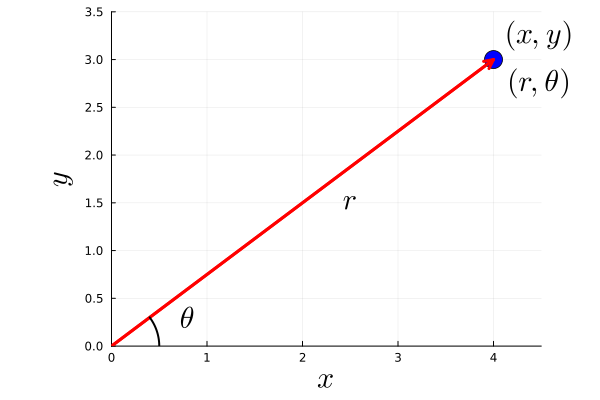
\includegraphics[width=0.45\columnwidth]{graphics/Chap07/PolarCoordinates.png}}%
% \hspace{5pt}%
% \subfloat[]{%
%     %\label{fig:MonotonicB}%
% 	\centering
% 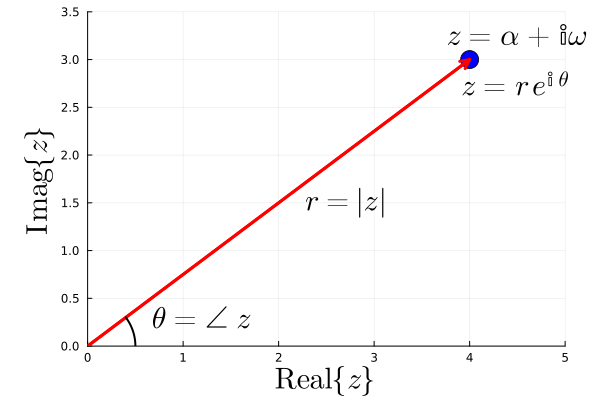
\includegraphics[width=0.45\columnwidth]{graphics/Chap07/PolarCoordinatesComplexCase.png}}%
%     \caption[]{Polar Coordinates. (a) in the real plane and (b) in the complex plane. Note, to reliably compute the angle, $\theta$, you \textbf{should NOT use the standard arctangent command} because it only works for $x>0$ and ${\rm Real }(z)>0$. Instead, use $\atan2(x,y)$ or ${\rm angle}(z)$ as explained in the text.}
%     \label{fig:PolarCoordiantesComplexNumbers}
% \end{figure}

\subsubsection{Antiderivatives for a Pair of Complex Conjugate Roots}

The denominator of the real rational function 
$$R(x)=\frac{a x + b}{\left(x - \alpha\right)^2 + \omega^2}$$
has complex roots, $z= \alpha + \im \omega$ and $z^\ast = \alpha - \im \omega $, where $z^\ast$ is the \textbf{complex conjugate} of $z$. While it is true that $R(x)$ can be expanded as
$$R(x) = \frac{\kappa}{x-z} + \frac{\kappa^\ast}{x-z^\ast},$$
trying to find the antiderivative in this form would take us into the realm of the Calculus of Complex Variables, which is beyond the scope of the course. Instead, we work directly with $R(x)$ as a ratio of a linear numerator and a quadratic denominator.

\bigskip

\begin{propColor}{Antiderivative for a Pair of Complex Conjugate Roots}{PairComplexConjugateRoots}

Consider a real rational function $R(x) = \frac{a x + b}{\left(x - \alpha\right)^2 + \omega^2}$. Its antiderivative is,
\begin{equation}
\label{eq:AntiderivativeRationalPairComplexConjugateRoots}
    \int \frac{a x + b}{(x - \alpha)^2 + \omega^2} \, dx = \frac{a}{2} \ln\left((x - \alpha)^2 + \omega^2\right) + \left(b - a\alpha\right) \frac{1}{\omega} \arctan\left(\frac{xs - \alpha}{\omega}\right) + C,
\end{equation}
where $C$ is a constant of integration. 

\end{propColor}

\textbf{Proof:} The antiderivative of the function \(\frac{ax + b}{(x-\alpha)^2 + \omega^2}\) is found by combining u-substitution and the recognition of a total derivative. The integral is broken down into two parts based on the numerator,
\[
\int \frac{ax + b}{(x-\alpha)^2 + \omega^2} \, dx = \int \frac{a(x-\alpha) + (a\alpha + b)}{(x-\alpha)^2 + \omega^2} \, dx,
\]
where splitting the integral gives,
\[
= a\int \frac{x-\alpha}{(x-\alpha)^2 + \omega^2} \, dx + (a\alpha + b)\int \frac{1}{(x-\alpha)^2 + \omega^2} \, dx.
\]

\textbf{Step 1: Using u-Substitution:}

For the first part,
\[
a\int \frac{x-\alpha}{(x-\alpha)^2 + \omega^2} \, dx,
\]
we let \(u = (x-\alpha)^2 + \omega^2\), then \(du = 2(x-\alpha)dx\), and \(\frac{1}{2}du = (x-\alpha)dx\). Thus, this part of the integral becomes,
\[
\frac{a}{2}\, \int \frac{1}{u} du = \frac{a}{2} \, \ln|u| + C_1 = \frac{a}{2}\ln\left( (x-\alpha)^2 + \omega^2 \right) + C_1
\]
after substituting back in $u = (x-\alpha)^2 + \omega^2$. Because $ (x-\alpha)^2 + \omega^2 > 0$, the absolute value can be removed; indeed, if $\omega = 0$, then the root is not complex.\\

\textbf{Step 2: Recognizing the Derivative of Arctangent} 

For the second part,
\[
(a\alpha + b)\int \frac{1}{(x-\alpha)^2 + \omega^2} \, dx,
\]
is a total differential of the arctangent function, namely,
\[
\frac{a\alpha + b}{\omega}\arctan\left(\frac{x-\alpha}{\omega}\right) + C_2,
\]
where once again, we used the fact that because the root is complex, $\omega$ cannot equal zero.\\

\textbf{Final Step:}

Combining both parts, we get the full antiderivative,
\[
\int \frac{ax + b}{(x-\alpha)^2 + \omega^2} \, dx = \frac{a}{2}\ln \left((x-\alpha)^2 + \omega^2 \right) + \frac{a\alpha + b}{\omega}\arctan\left(\frac{x-\alpha}{\omega}\right) + C
\]
where \(C := C_1 + C_2\) is the constant of integration. 
\Qed

\bigskip

\begin{example} Find an antiderivative for $R(x) = \frac{2x+1}{3 x^2 -6 x + 15}$.    
\end{example}

\solution \Ans ~~$\frac{1}{3}\cdot \log\left( x^{2} - 2 \cdot x + 5 \right) + \frac{1}{2} \cdot \arctan\left( \frac{x}{2} - \frac{1}{2} \right)$\\

We identify $P(x) = 2x+1$ and $Q(x) = 3 x^2 -6 x +15$, which clearly satisfy the degree of the numerator being less than the degree of the denominator. To see if the denominator has real or complex poles, we check the discriminant
$$b^2 - 4 ac = (-6)^2 - 4(3)(15) = -144 < 0,$$ 
and hence, the roots are complex. Indeed, applying the quadratic formula yields $z=1 \pm 2\im$, and thus
$$\alpha=1 \quad \text{and} \quad \omega = 2;$$
it is fine to chose $\omega = -2$ as it will not change the answer.\\

The final step for applying Proposition~\ref{thm:PairComplexConjugateRoots} is to make the denominator monic by factoring out the coefficient of $x^2$,
$$R(x) = \frac{1}{3} \cdot \frac{2 x + 1}{x^2 - 2 x + 5}=  \frac{1}{3} \cdot \frac{2 x + 1}{(x-1)^2 + 2^2}.$$
Substituting into \eqref{eq:AntiderivativeRationalPairComplexConjugateRoots} yields,

$$\int R(x)\, dx = \frac{1}{3} \cdot \left(\log\left( x^{2} - 2 \cdot x + 5 \right) + \frac{3 \cdot \arctan\left( \frac{x}{2} - \frac{1}{2} \right)}{2} \right).$$
\Qed


% Handling distinct complex roots is almost as easy as handling distinct real roots, once one is equipped with a few facts about complex numbers. However, the algebra can be even more tedious, further highlighting the need for software intervention! The key property we need is a complex equivalent of polar coordinates as illustrated in Fig.~\ref{fig:PolarCoordiantesComplexNumbers}. Even for (real) Cartesian coordiantes, students typically struggle with computing the angle. This problem goes away if you use the function ${\rm atan2}(x,y)$ instead of the standard arctangent of a ratio. Why? 
% \begin{itemize}
%     \item \textbf{Quadrant Awareness:} Unlike ${\rm atan}(y/x)$, which only returns values between $-\frac{\pi}{2}$ and $\frac{\pi}{2}$, ${\rm atan2}(x,y)$ correctly identifies the quadrant of the point, returning values in the range $(-\pi, \pi]$. This eliminates ambiguity in angle determination.
   
%     \item \textbf{Division by Zero Handled:} Directly computing \texttt{atan(y/x)} can lead to division by zero if \(x = 0\). ${\rm atan2}$ handles this gracefully, returning $\frac{\pi}{2}$ or $-\frac{\pi}{2}$ as appropriate.
   
%     \item \textbf{Precision and Performance:} ${\rm atan2}$ is optimized for accuracy and computational efficiency, making it ideal for high-performance computing applications.
% \end{itemize}



% \begin{factColor}{Complex Numbers have a Magnitude and a Phase Angle}{ComplexNumbersMagnitudePhase}
%  Let $\alpha$ and $\omega$ be real numbers, and let $\im$ be the imaginary unit (aka, $\im = \sqrt{-1})$. Then the following hold:

%    \begin{enumerate}
%    \renewcommand{\labelenumi}{(\alph{enumi})}
% \setlength{\itemsep}{.2cm}
%        \item $z := \alpha + \im \omega\in \cp$ is a Cartesian representation of a complex number.
%        \item $|z|:=\sqrt{\alpha^2 + \omega^2}$ is the \textbf{magnitude} of $z$.
%        \item $\theta:= \angle z = {\rm atan2}(\alpha, \omega)$ is the \textbf{angle} of $z$.
%        \item $z = |z| \, e^{\im \theta} = |z|\, \left( \cos(\omega) + \im \sin(\omega) \right)$ by Euler's Formula. It is called the \textbf{exponential form or Euler's form} of the complex number.
%        \item A common shorthand notation is to write $z = |z|\, e^{\im \angle z}$, which obviates the need to define a new variable, $\theta$.
%        \item $z^\ast:=\alpha - \im \omega$ is the \textbf{complex conjugate} of $z$. It satisfies, $z^\ast =  |z|\, e^{-\im \angle z}$, meaning, it has the same magnitude as $z$ and opposite phase angle.
%    \end{enumerate}
% \end{factColor}

% \bigskip



% \begin{lstlisting}[language=Julia,style=mystyle]
% using Printf

% # Define atan2 in terms of the angle function for complex numbers
% # While standard in most languages, Julia uses the angle function for complex numbers
% atan2(x, y) = angle(x + y*im)

% # Define the complex number z = alpha + i*omega
% alpha, omega = -3, 4

% # Convert to polar coordinates using the newly defined atan2
% r = sqrt(alpha^2 + omega^2)
% theta = atan2(alpha, omega) # Using the custom atan2 definition

% # Explanations
% println("Given alpha = $(alpha), omega = $(omega)")
% println("a) Cartesian representation of z: $(alpha) + $(omega)i")
% println("b) Magnitude of z (|z|): $(r)")
% println("c) Angle of z using custom atan2 (theta): $(theta) radians")

% # Compare with Julia's angle function directly
% theta_angle = angle(alpha + omega*im)
% println("\nUsing Julia's angle function directly for comparison:")
% println("Angle of z using angle(z): $(theta_angle) radians")

% # Note on atan(y/x) vs atan2(x, y) vs angle(z)
% println("\nNote: While atan(y/x) can lead to ambiguities due to quadrant,")
% println("our custom atan2(x, y) and Julia's angle(z) correctly account for the quadrant,")
% println("ensuring the angle is determined accurately for complex numbers.")
% \end{lstlisting}
% \textbf{Output} 
% \begin{verbatim}
% Given alpha = -3, omega = 4
% a) Cartesian representation of z: -3 + 4i
% b) Magnitude of z (|z|): 5.0
% c) Angle of z using custom atan2 (theta): 2.214297435588181 radians

% Using Julia's angle function directly for comparison:
% Angle of z using angle(z): 2.214297435588181 radians

% Note: While atan(y/x) can lead to ambiguities due to quadrant,
% our custom atan2(x, y) and Julia's angle(z) correctly account for the quadrant,
% ensuring the angle is determined accurately for complex numbers.
% \end{verbatim}

%\bigskip

\subsubsection{Antiderivatives for a Mixture of Real and Complex Conjugate Roots}

As you are well aware, real polynomials often have a mixture of real roots and complex roots, with the complex roots occurring in complex conjugate pairs. Pairs of complex conjugate roots can be recombined to give a quadratic polynomial with real coefficients, which can then be integrated as in the previous subsection. We'll first show how the corresponding partial fraction expansions work in software, and then we'll state, for the record, the corresponding theoretical result.\\

\begin{example}
\label{ex:6thOrderDenominator}
Use software to find first the partial fraction expansion and then the antiderivative of
$$R(x) = \frac{2 \cdot x^{3} - x + 4}{x^{6} - 4 \cdot x^{4} + 10 \cdot x^{3} - 11 \cdot x^{2} + 10 \cdot x - 6}. $$   
Clearly, doing this by hand would be a nightmare. You already need an algorithm to find the roots of the denominator, so why not use another algorithm to find the coefficients in the PFE? 
\end{example}

\begin{lstlisting}[language=Julia,style=mystyle]
using SymPy

# Define the variable
x = symbols("x")

P = 2*x^3 - x + 4
Q = x^6 - 4*x^4 + 10*x^3 - 11*x^2 + 10*x - 6

R = P/Q

# Compute the PFE
PFE = apart(R)

println(PFE)
\end{lstlisting}
\textbf{Output} 
\begin{verbatim}
-(4*x + 3)/(10*(x^2 + 1)) - (5*x - 8)/(17*(x^2 - 2*x + 2)) + 47/(680*(x + 3)) + 5/(8*(x - 1))
\end{verbatim}
or, nicely typeset,
$${\rm PFE}(x) =  \frac{ - \left( 4 \cdot x + 3 \right)}{10 \cdot \left( x^{2} + 1 \right)} - \frac{5 \cdot x - 8}{17 \cdot \left( x^{2} - 2 \cdot x + 2 \right)} + \frac{47}{680 \cdot \left( x + 3 \right)} + \frac{5}{8 \cdot \left( x - 1 \right)}$$
The \texttt{apart} function in \texttt{SymPy} has nicely expanded the rational function as a sum of first-order terms and second-order terms. We could not ask for more, because we know how antiderivatives for each term! But instead of doing them by hand, we continue with software.

\bigskip
\textcolor{blue}{\bf \Large Continuing with the antiderivative:}\\


\begin{lstlisting}[language=Julia,style=mystyle]
antiderivative = integrate(PFE, x)
println(antiderivative)
\end{lstlisting}
\textbf{Output} 
\begin{verbatim}
5*log(x - 1)/8 + 47*log(x + 3)/680 - log(x^2 + 1)/5 - 5*log(x^2 - 2*x + 2)/34 
- 3*atan(x)/10 + 3*atan(x - 1)/17
\end{verbatim}
or nicely typeset,
$$\int R(x)\, dx =\frac{5 \cdot \log\left( x - 1 \right)}{8} + \frac{47 \cdot \log\left( x + 3 \right)}{680} - \frac{\log\left( x^{2} + 1 \right)}{5} - \frac{5 \cdot \log\left( x^{2} - 2 \cdot x + 2 \right)}{34} - \frac{3 \cdot \arctan\left( x \right)}{10} + \frac{3 \cdot \arctan\left( x - 1 \right)}{17}. $$

\bigskip
\textcolor{blue}{\bf \Large As you might guess, the antiderivative can also be computed in one step, in other words, without first doing a PFE:}\\

\begin{lstlisting}[language=Julia,style=mystyle]
# Find the antiderivative of the rational function
antiderivative = integrate(R, x)
println(antiderivative)
\end{lstlisting}
\textbf{Output} 
\begin{verbatim}
5*log(x - 1)/8 + 47*log(x + 3)/680 - log(x^2 + 1)/5 - 5*log(x^2 - 2*x + 2)/34 
- 3*atan(x)/10 + 3*atan(x - 1)/17
\end{verbatim}
or nicely typeset,
$$\int R(x)\, dx =\frac{5 \cdot \log\left( x - 1 \right)}{8} + \frac{47 \cdot \log\left( x + 3 \right)}{680} - \frac{\log\left( x^{2} + 1 \right)}{5} - \frac{5 \cdot \log\left( x^{2} - 2 \cdot x + 2 \right)}{34} - \frac{3 \cdot \arctan\left( x \right)}{10} + \frac{3 \cdot \arctan\left( x - 1 \right)}{17}. $$

\Qed


\bigskip 

\textcolor{blue}{\bf \Large Below is how the subject is taught (if at all) in a traditional Calculus course.}

\bigskip

\begin{propColor}{(Optional Read:) Antiderivative for a Mixture of Real and Complex Roots}{AntiderivativeMixedRealComplexRoots}

Consider a real rational function $R(x) = \frac{P(x)}{Q(x)}$ where the degree of the numerator is strictly lower than the degree of the denominator, $Q(x)$ is monic, and the roots of the denominator polynomial are distinct. We list the roots as
\begin{itemize}
    \item \textbf{real roots:} $r_1$, $r_2$, $\ldots$, $r_m$
    \item \textbf{complex roots:} $z_1$, $z_2$, $\ldots$, $z_p$ followed by their \textbf{complex conjugates}, $z_1 ^\ast$, $z_2 ^\ast$, $\ldots$, $z_p ^\ast$, where
    \item ${\rm Real}\{z_i\} =: \alpha_i$ and  ${\rm Imag}\{z_i\} =: \omega_i$, so that $z_i = \alpha_i + \im \omega_i$.
\end{itemize}
Under these assumptions,
$$ Q(x) = \prod_{i=1}^p (x - z_i)(x-z_i^\ast) = \prod_{i=1}^p \left( \left(x - \alpha_i\right)^2 + \omega_i^2 \right),$$
and the rational function $R(x)$ can be expressed as a partial fraction expansion (PFE)
$$R(x) = \sum_{i=1}^m \frac{k_i}{x - r_i} + \sum_{i=1}^p \frac{a_i x + b_i}{(x - \alpha_i)^2 + \omega_i^2},$$
where the real coefficients $k_i, a_i, b_i$ satisfy
\begin{equation}
    k_i = \lim_{x \to r_i} \frac{(x-r_i) P(x)}{Q(x)} = \frac{P(r_i)}{\prod_{\substack{j=1 \\ j \neq i}}^n (r_i-r_j)},
\end{equation}
for the real roots, and for the complex roots,
\begin{equation}
\begin{aligned}
     a_i &= {\rm Real}\left\{ \lim_{x \to z_i} \frac{(x - z_i)P(x)}{Q(x)} \right\} = {\rm Real}\left\{ \frac{P(z_i)}{(z_i-z_i^\ast)}  \cdot \frac{1}{\prod_{\substack{j=1 \\ j \neq i}}^p \left( \left(z_i - \alpha_j\right)^2 + \omega_j^2 \right)}\right\}, \\[1em]
     b_i &= {\rm Imag}\left\{ \lim_{x \to z_i} \frac{(x - z_i)P(x)}{Q(x)} \right\} =  {\rm Imag}\left\{ \frac{P(z_i)}{(z_i-z_i^\ast)}  \cdot \frac{1}{\prod_{\substack{j=1 \\ j \neq i}}^p  \left( \left(z_i - \alpha_j\right)^2 + \omega_j^2 \right)}\right\}.
\end{aligned}
\end{equation}
\bigskip

\textbf{Antiderivative of a Generic Term:} The antiderivative for a term of the form $\frac{k}{x-r}$ can be found as follows:
\begin{equation}
    \int \frac{k}{x-r} \, dx =  k \ln|x-r| + C,
\end{equation}
where $C$ is the integration constant.\\


\textbf{Antiderivative of a Generic Term:} The antiderivative for a term of the form $\frac{a x + b}{(x - \alpha)^2 + \omega^2}$ can be found as follows:
\begin{equation}
    \int \frac{a x + b}{(x - \alpha)^2 + \omega^2} \, dx = \frac{a}{2} \ln\left((x - \alpha)^2 + \omega^2\right) + \left(b - a\alpha\right) \frac{1}{\omega} \arctan\left(\frac{xs - \alpha}{\omega}\right) + C,
\end{equation}
where $C$ is the integration constant.  
\end{propColor}

\bigskip

\emstat{We do not offer practice videos because doing partial fraction expansions by hand is a fool's errand for anything but the simplest of cases.  It's advisable to employ software tools for calculating PFEs for anything other than a second-order problem, and once you do that, why not go ahead and compute the antiderivative using software as well? }





\subsection{Trigonometric Substitutions for Radicals}
\label{sec:trigSubstitutions}

Trigonometric substitution is a technique for computing antiderivatives (and integrals) that is particularly useful when the integrand involves expressions like \( \sqrt{a^2 - x^2} \), \( \sqrt{a^2 + x^2} \), or \( \sqrt{x^2 - a^2} \). Here, we carefully work out examples where trigonometric substitution is commonly used, highlighting common pitfalls along the way. 

\bigskip
\textbf{Heads up:} Trig substitution is the most technically and mentally taxing of all the methods for finding antiderivatives by hand. Hence, if you find it difficult, you are not alone. You might see it a few times in an engineering course, though it arises less frequently than u-substitution and integration by parts. We will include images that help you to understand how the transformations were ``discovered''.
\bigskip

\begin{center}
    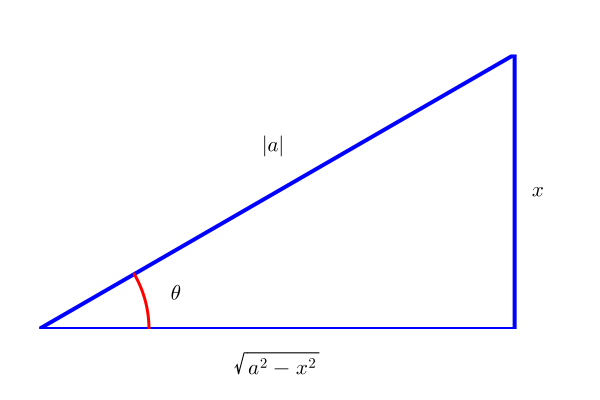
\includegraphics[width=0.6\columnwidth]{graphics/Chap07/TrigSubSqRtAsqMinusXsq.png}
\end{center}

The above triangle satisfies the Pythagorean Theorem, and hence, it is a right triangle. From basic trigonometry it follows that the opposite side of the triangle is given by $x = |a| \sin(\theta)$, which motivates the change of variable we use in the next problem. \\

\begin{example}
\label{ex:aSquaredMinusXsquared}
    Evaluate $ \int \sqrt{a^2 - x^2} \, dx.$
\end{example}

\solution Ans. For $|x| \le |a|$, $\int \sqrt{a^2 - x^2} \, dx =  \frac{a^2}{2} \cdot \arcsin\left(\frac{x}{|a|} \right) + \frac{x}{2} \cdot \sqrt{a^2 - x^2} + C$.

Because $a$ is squared in the integrand, we can either replace it by $|a|$ or simply assume that $a > 0$. We'll make fewer errors if we use $|a|$, as in the diagram.  \\

The integrand exists and is continuous for $(a^2 - x^2 \ge 0) \iff (-|a| \le x \le |a|)$. The standard trig substitution for this integral is  \(x = |a| \sin(\theta) \) and  \( dx = |a| \cos(\theta) \, d\theta \). We note that with $ -\frac{\pi}{2} \le \theta \le \frac{\pi}{2}$, it follows that $-|a| \le x \le |a|$ and that $0 \le \cos(\theta) \le 1$. Moreover, later, when we need to inverse the transformation, we are working with a principal domain for defining $\arcsin(x)$. Hence, everything checks out!\\

Using this substitution and recalling that $1 - \sin^2(x) = \cos^2(x)$, the integral becomes
\begin{align*}
    \int \left( \sqrt{a^2 - a^2 \sin^2(\theta)} \right) \cdot |a| \cos(\theta) \, d\theta & =  \int \left( \sqrt{a^2\cdot  \cos^2(\theta)} \right) \cdot |a| \cos(\theta) \, d\theta \\[1em]
    & = \int \left( |a| \cdot  |\cos(\theta)| \right) \cdot |a| \cos(\theta) \, d\theta \\[1em]
    &= a^2 \int \cos^2(\theta)\, d\theta
\end{align*}
where the last equality follows because we (carefully) noted earlier that $\cos(\theta)\ge 0$ for $ -\frac{\pi}{2} \le \theta \le \frac{\pi}{2}$, the domain where the substitution was defined.\\

\emstat{\textbf{A visual derivation based on the triangle:} From $x =|a| \sin(\theta)$, we deduce that $dx = |a| \cos(\theta) \, d\theta$. We also have the adjacent side of the triangle is $|a| \cos(\theta) = \sqrt{a^2 - x^2}$, which can be used to simplify the integrand. Substituting these into the integral, we have
$$ \int \sqrt{a^2 - x^2} \, dx = \int \underbrace{|a| \cos(\theta)}_{\sqrt{a^2 - x^2}} \cdot \underbrace{|a| \cos(\theta) \, d\theta}_{dx} =  a^2 \int \cos^2(\theta)\, d\theta.$$}

Using the half-angle identity, \( \cos^2(\theta) = \frac{1 + \cos(2\theta)}{2} \), we have
\[
a^2 \int \cos^2(\theta)\, d\theta = \frac{a^2}{2} \int (1 + \cos(2\theta)) \, d\theta = \frac{a^2}{2} \left( \theta + \frac{\sin(2\theta)}{2} \right) + C.
\]
To return to \( x \), we use \( \sin(\theta) = \frac{x}{|a|} \) and \( \cos(\theta) = \sqrt{1 - \sin^2(\theta)} = \sqrt{1 - \left(  \frac{x}{|a|}\right)^2}\). Importantly, as noted earlier, we are working with a principal domain of the function $\arcsin$. Thus
\[
\theta = \arcsin\left(\frac{x}{a}\right),~\text{and}~\sin(2\theta) = 2\sin(\theta)\cos(\theta) = \frac{2x}{|a|}\sqrt{1 - \left(\frac{x}{|a|}\right)^2}.
\]
The final antiderivative in terms of \( x \) is
\[
\int \sqrt{a^2 - x^2} \, dx = \frac{a^2}{2} \left( \arcsin\left(\frac{x}{|a|}\right) + \frac{x}{|a|}\sqrt{1 - \left(\frac{x}{|a|}\right)^2} \right) + C.
\]
Because $-1 \le \frac{x}{|a|} \le 1$ for all $x$ in the domain of the integrand, the terms $\arcsin\left(\frac{x}{|a|} \right)$ and $\sqrt{1 - \left(\frac{x}{|a|}\right)^2}$ in the antiderivative are well defined (i.e., make mathematical sense\footnote{As an example, if $\frac{x}{|a|}$ were greater than one, then neither the arcsine nor the square root would make sense.}); hence, the computed antiderivative is defined for all $x$ in the domain of the integrand.\\

A more aesthetically pleasing form of the answer can be obtained with a small bit of algebra, 
\[
\setlength{\fboxrule}{2pt} % Adjust the thickness of the border
\fcolorbox{brightblue}{lightblue}{%
\addtolength{\fboxsep}{5pt} % Padding around the formula
For $|x|\le |a|$, $\displaystyle
\int \sqrt{a^2 - x^2} \, dx =  \frac{a^2}{2} \cdot \arcsin\left(\frac{x}{|a|} \right) + \frac{x}{2} \cdot \sqrt{a^2 - x^2} + C.
$%
}
\]

\textbf{Note:} From the right triangle associated with this problem, we have $\theta = \arcsin\left(\frac{x}{|a|}\right)$ and $\theta =\atan\left(\frac{x}{\sqrt{a^2 - x^2}}\right)$, and thus 
$$ \arcsin\left(\frac{x}{|a|}\right) =\atan\left(\frac{x}{\sqrt{a^2 - x^2}}\right). $$ It follows that the answer can also be written as 
\[
\setlength{\fboxrule}{2pt} % Adjust the thickness of the border
\fcolorbox{brightblue}{lightblue}{%
\addtolength{\fboxsep}{5pt} % Padding around the formula
For $|x|\le |a|$, $\displaystyle
\int \sqrt{a^2 - x^2} \, dx =   \frac{a^2}{2} \cdot \atan\left(\frac{x}{\sqrt{a^2 - x^2}}\right) + \frac{x}{2} \cdot \sqrt{a^2 - x^2} + C.
$%
}
\]
\Qed
\bigskip


%%%%%%%%%%%%%%%%%%%%%%%%%%%%%%%%%%%%%%%%%%%%%%%%

\begin{center}
    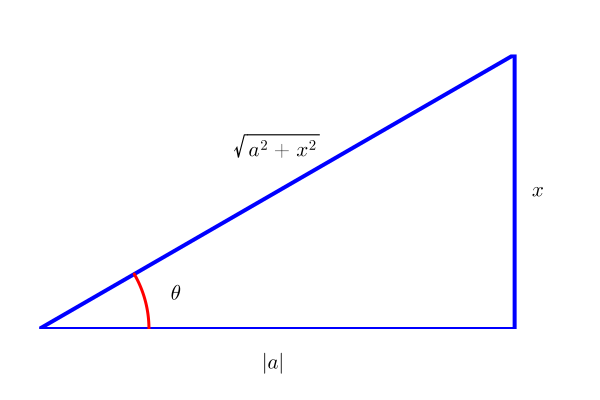
\includegraphics[width=0.6\columnwidth]{graphics/Chap07/TrigSubSqRtAsqPlusXsq.png}
\end{center}

Note that the above triangle satisfies the Pythagorean Theorem, and hence it is a right triangle. It follows that $\tan(\theta) =  \frac{x}{|a|}$, or, $x = |a| \tan(\theta)$, which motivates the change of variable we use in the next problem. \\


\begin{example} Evaluate the integral
\[
\int \sqrt{a^2 + x^2} \, dx.
\]    
\end{example}

\solution Ans. For $x \in \real$, $\int \sqrt{a^2 + x^2} \, dx =  \frac{a^2}{2}\ln \left(x +  \sqrt{a^2 + x^2 } \right) +   \frac{x}{2} \cdot \sqrt{a^2 + x^2} +C$.\\

The integrand $\sqrt{a^2 + x^2} \, dx$ is defined and continuous in $(-\infty, \infty)$. Because $a$ is squared, we replace it by $|a|$ to avoid sign errors later on.\\

The substitution \( x = |a| \tan(\theta) \)  is defined for $ -\frac{\pi}{2} < \theta < \frac{\pi}{2}$, and gives  \( dx = |a| \cdot \sec^2(\theta) \, d\theta \). The integral becomes
\[
\int \sqrt{a^2 + a^2 \tan^2(\theta)} \cdot  |a| \cdot \sec^2(\theta) \, d\theta =  \int \sqrt{a^2 \left(1 + \tan^2(\theta) \right)}\cdot  |a| \cdot \sec^2(\theta) \, d\theta.
\]
%% = a^2 \int \sec^3(\theta) \, d\theta
Next, we use the trig identity,  $1 + \tan^2(\theta) = \sec^2(\theta)$, giving us 
\begin{align*}
    \int \sqrt{a^2 \left(1 + \tan^2(\theta) \right)}\cdot  |a| \cdot \sec^2(\theta) \, d\theta & = \int \sqrt{a^2 \cdot \sec^2(\theta)} \cdot  |a| \cdot \sec^2(\theta) \, d\theta \\[1em] 
    &= \int |a| |\sec(\theta)| \cdot  |a| \cdot \sec^2(\theta) \, d\theta \\[1em]
    & = a^2  \int \sec^3(\theta) \, d\theta
\end{align*}
where in the last line we used the fact that $\sec(\theta):=\frac{1}{\cos(\theta)}$ is positive for $ -\frac{\pi}{2} < \theta < \frac{\pi}{2}$, the domain of the change of variable.\\


%The first integral, \( \int \sec(\theta) \, d\theta \), was worked in Eaxmple~\ref{ex:TrickySecant}, with solution \( \ln|\sec(\theta) + \tan(\theta)| \). \\

\textbf{Computing the antiderivative of  $\bm{ \mathrm{\bf \int} \sec^3(\theta) \, d\theta}$ requires a new technique that is useful to know when performing integration by parts.} Define,
\begin{equation}
\label{eq:antiderivativeSecCubed}
\begin{aligned}
    I &:=  \int \sec^3(\theta) \, d\theta \\[1em]
    &= \int  \sec(\theta)  \cdot \left( 1 + \tan^2(x) \right)\, d\theta ~~(~\text{trig identity,}~~  1 + \tan^2(\theta) = \sec^2(\theta)~)\\[1em]
    & =  \int  \sec(\theta) \, d\theta +  \int  \sec(\theta)  \cdot  \tan^2(x) \, d\theta ~~(~\text{algebra} ) \\[1em] 
    & =  \ln|\sec(\theta) + \tan(\theta)| + \int  \sec(\theta)  \cdot  \tan^2(x) \, d\theta ~~(\text{first integral is from Example~\ref{ex:TrickySecant}}).
\end{aligned}    
\end{equation}
The remaining integral in \eqref{eq:antiderivativeSecCubed} requires integration by parts. Define 
\begin{align*}
    u &= \tan(\theta)  \implies  du = \sec^2(\theta) \, d\theta \\
    v& = \sec(\theta)  \implies  dv = \sec(\theta) \cdot \tan(\theta) \, d\theta , 
\end{align*}
yielding,
\begin{equation}
\label{eq:antiderivativeSecCubedStep2}
\begin{aligned}
    \int \underbrace{\sec(\theta) \tan^2(\theta) \, d\theta}_{u\, dv} &= \underbrace{\tan(\theta) \sec(\theta)}_{u\cdot v} - \int \underbrace{\sec(\theta) \sec^2(\theta) \, d\theta}_{v \, du} \\[1em]
    & = \tan(\theta) \sec(\theta) - \int \sec^3(\theta) \, d\theta \\[1em]
    & =  \tan(\theta) \sec(\theta) - I.
\end{aligned}
\end{equation}

Substituting back into \eqref{eq:antiderivativeSecCubed}, we have
\begin{equation}
\label{eq:antiderivativeSecCubedStep3}
\begin{aligned}
    I:=  \int \sec^3(\theta) \, d\theta   & =  \ln|\sec(\theta) + \tan(\theta)| + \int  \sec(\theta)  \cdot  \tan^2(x) \, d\theta \\[1em]
    &= \ln|\sec(\theta) + \tan(\theta)| + \tan(\theta) \sec(\theta) - I.
\end{aligned}  
\end{equation}
Solving for $I$ yields
\begin{equation}
\label{eq:antiderivativeSecCubedStep4}
\begin{aligned}
    2 I &=  \ln|\sec(\theta) + \tan(\theta)| + \tan(\theta) \sec(\theta) \\
    & \Downarrow \\
    I &= \frac{1}{2}  \ln|\sec(\theta) + \tan(\theta)| + \frac{1}{2} \tan(\theta) \sec(\theta). 
\end{aligned}  
\end{equation}

Putting the (numerous) steps together yields
$$ \int \sqrt{a^2 + x^2} \, dx = a^2  \int \sec^3(\theta) \, d\theta = a^2 I =  \frac{a^2}{2}  \ln|\sec(\theta) + \tan(\theta)| + \frac{a^2}{2} \tan(\theta) \sec(\theta).$$

To return to an answer in \( x \) , we use the trigonometric substitutions,
\begin{align*}
\tan(\theta) &= \frac{x}{|a|}, \\
\sec(\theta) &=  \sqrt{1 + \tan^2(\theta)}  = \sqrt{1 + \left(\frac{x}{|a|}\right)^2}.
\end{align*}
The final antiderivative in terms of \( x \) is
\begin{align*}
    \int \sqrt{a^2 + x^2} \, dx & = \frac{a^2}{2}  \ln\left| \sqrt{1 + \left(\frac{x}{|a|}\right)^2} + \frac{x}{|a|}\right| + \frac{a^2}{2}  \frac{x}{|a|}\cdot\sqrt{1 + \left(\frac{x}{|a|}\right)^2} +C \\[1em]
    &=    \frac{a^2}{2}  \ln\left(\sqrt{1 + \left(\frac{x}{|a|}\right)^2} + \frac{x}{|a|}\right) + \frac{x}{2} \cdot \sqrt{a^2 + x^2} +C 
\end{align*}
where \( C \) is the constant of integration. The absolute value signs in the natural logarithm were removed because 
$$\sqrt{1 + \left(\frac{x}{|a|}\right)^2} + \frac{x}{|a|} >0$$
for all $x \in \real$.\\

It is traditional to simplify further the answer by taking advantage of the arbitrary constant of integration, $C$.
\begin{align*}
  \ln\left(\sqrt{1 + \left(\frac{x}{|a|}\right)^2} + \frac{x}{|a|}\right)  &= \ln\left( \frac{1}{|a|} \cdot \left( \sqrt{a^2 + x^2 } + x \right) \right)\\[1em]
 & = \ln \left( \frac{1}{|a|} \right) + \ln \left( \sqrt{a^2 + x^2 } + x \right) \\[1em]
\end{align*}
Absorbing the constant $\ln \left( \frac{1}{|a|} \right)$ into $C$ gives a much nicer final answer, 
\[
\setlength{\fboxrule}{2pt} % Adjust the thickness of the border
\fcolorbox{brightblue}{lightblue}{%
\addtolength{\fboxsep}{5pt} % Padding around the formula
For $x\in \real$, $\displaystyle
\int \sqrt{a^2 + x^2} \, dx =  \frac{a^2}{2}\ln \left(x +  \sqrt{a^2 + x^2 } \right) +   \frac{x}{2} \cdot \sqrt{a^2 + x^2} +C.
$%
}
\]


\textbf{Note:} The answer looks so innocent. Why was it so hard to compute? 

\Qed


%%%%%%%%%%%%%%%%%%%%%%%%%%%%%%%%%%%%%%%%%%%%%%%%

\begin{center}
    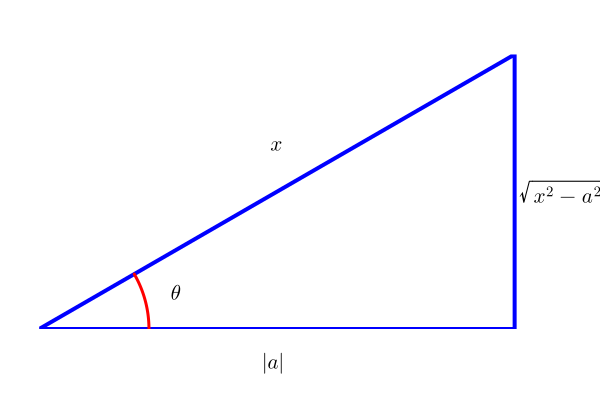
\includegraphics[width=0.6\columnwidth]{graphics/Chap07/TrigSubSqRtXsqMinusAsq.png}
\end{center}

Note that the above triangle satisfies the Pythagorean Theorem, and hence it is a right triangle. It follows that $\cos(\theta) =  \frac{|a|}{x}$, or, $x = \frac{|a|}{\cos(\theta)} = |a| \sec(\theta)$, which motivates a common change of variables for the next problem. There is also another viable change of variable that we wish to illustrate. \textcolor{blue}{\bf Hyperbolic Trig Functions} are often used in integrals that have terms of the form \( x^2 - a^2 \). This is because of identities such as, $\cosh^2(x) - \sinh^2(x) = 1$, which can also be written as $\cosh^2(x) - 1 = \sinh^2(x)$. This next example follows a similar pattern to the previous examples, ensuring that the domain of the integrand is carefully delineated and each change of variables respects the domain in which the integrand is defined.

\bigskip
\begin{example}
 Find an antiderivative for  \( \sqrt{x^2 - a^2} \).
\end{example}

\solution Ans. For $|x|\ge |a|$, $\int \sqrt{x^2 - a^2}\, dx = \frac{x}{2}\sqrt{x^2 - a^2} - \operatorname{sign}(x) \cdot \frac{a^2}{2} \ln\left( |x| + \sqrt{x^2 - a^2} \right) + C$, where 
$$ \operatorname{sign}(x) = \begin{cases}
    +1 & x \ge 0 \\
    -1 & x<0.     
\end{cases}$$

\textcolor{blue}{\bf First Approach: Standard Trig Substitution:} The integrand of \( \int \sqrt{x^2 - a^2} \, dx \) is defined and continuous wherever \( x^2 - a^2 \ge 0 \), that is \( |x| \ge |a| \). We can therefore develop an antiderivative for $x \ge |a|$, and a second one for $x \le -|a|$. Here, we will develop a solution for $x \le -|a|$ using standard trig functions, and with the hyperbolic trig functions, we'll develop the solution for $x \ge |a|$.\\


For $x \le - |a|$, we choose the change of variable \( x = -|a| \sec(\theta) \), which gives \( dx = -|a| \sec(\theta)\cdot \tan(\theta) \, d\theta \). For all $0 \le \theta < \frac{\pi}{2}$, $ 1 \le \sec(\theta) < \infty$, and hence the change of variables respects the domain of definition of the integrand. Moreover, for later use, we note that for all $0 \le \theta < \frac{\pi}{2}$, $\tan(\theta) \ge 0$.\\

Using the change of variable, the integral becomes
\begin{align*}
   \int \sqrt{x^2 - a^2} \, dx  &=  \int \sqrt{a^2 \sec^2(\theta) - a^2} \cdot (-1)\cdot|a| \sec(\theta)\cdot \tan(\theta) \, d\theta\\[1em]
   &= -a^2 \int \sqrt{\tan^2(\theta)} \cdot \sec(\theta)\cdot \tan(\theta) \, d\theta ~~(\sec^2(\theta) - 1 = \tan^2(\theta)) \\[1em]
     &= -a^2 \int | \tan(\theta) | \cdot \sec(\theta)\cdot \tan(\theta) \, d\theta  ~~(\tan(\theta) \ge 0)\\[1em]
    &= -a^2 \int \tan^2(\theta) \cdot \sec(\theta) \, d\theta  ~~(\tan^2(\theta) = \sec^2(\theta) - 1)\\
    &= -a^2 \int \left( \sec^2(\theta) -1 \right)\cdot \sec(\theta) \, d\theta\\
     &=  - a^2 \int \sec^3(\theta) \, d\theta + a^2 \int \sec(\theta) \, d\theta.
\end{align*}


Fortunately for us, we have already computed antiderivatives for both of these integrands,
\begin{align*}
     \int \sec(\theta) \, d\theta &=  \ln|\sec(\theta) + \tan(\theta)| + C\\
      \int \sec^3(\theta) \, d\theta &=  \frac{1}{2}  \ln|\sec(\theta) + \tan(\theta)| + \frac{1}{2} \tan(\theta) \sec(\theta) +C.
\end{align*}
Hence, 
\begin{align*}
    \int \sqrt{x^2 - a^2} \, dx &=  - \frac{a^2}{2}  \ln|\sec(\theta) + \tan(\theta)| - \frac{a^2}{2} \tan(\theta) \sec(\theta) + a^2 \ln|\sec(\theta) + \tan(\theta)| +C \\[1em]
    &=   \frac{a^2}{2}  \ln|\sec(\theta) + \tan(\theta)| - \frac{a^2}{2} \tan(\theta) \sec(\theta)  +C 
\end{align*}

From $x = -|a| \sec(\theta)$, we have that $\sec(\theta) = - \frac{x}{|a|}$. From the trig diagram for the problem, we have
$$\tan(\theta)  = \frac{\sqrt{x^2 - a^2}}{|a|}.$$
Substituting in, we have 
\begin{align*}
\int \sqrt{x^2 - a^2} \, dx &= \frac{a^2}{2}  \ln \bigg|- \frac{x}{|a|} +  \frac{\sqrt{x^2 - a^2}}{|a|} \bigg| - \frac{a^2}{2} \frac{\sqrt{x^2 - a^2}}{|a|} \cdot \left(\frac{-x}{|a|}\right) +C \\[1em]
 &= \frac{a^2}{2}  \ln |-x + \sqrt{x^2 - a^2}| - \ln(|a|) + \frac{x}{2} \sqrt{x^2 - a^2} +C \\[1em]
 & = \frac{a^2}{2}  \ln |-x + \sqrt{x^2 - a^2}|+ \frac{x}{2} \sqrt{x^2 - a^2} +C,  
\end{align*}
where in the last line, we absorbed $ \ln(|a|)$ into the constant of integration, $C$.

\bigskip
\textcolor{blue}{\bf Second Approach: Hyperbolic Trig Functions:} The integrand of \( \int \sqrt{x^2 - a^2} \, dx \) is defined and continuous wherever \( x^2 - a^2 \ge 0 \), that is \( |x| \ge |a| \). We can therefore develop an antiderivative for $x \ge |a|$, and a second one for $x \le -|a|$.\\

For $x \ge |a|$, we choose the hyperbolic substitution \( x = |a| \cosh(t) \), which gives \( dx = |a| \sinh(t) \, dt \). For all $t\ge0$, $\cosh(t)\ge 1$, and hence the change of variables respects the domain of definition of the integrand. Moreover, for later use, we note that for all $t\ge 0$, $\sinh(t) \ge 0$.\\

%and \( t = \acosh\left(\frac{x}{|a|}\right) \), where \( \acosh\) is the inverse hyperbolic cosine function.

% \textbf{Note:} The the inverse hyperbolic cosine function, \( \acosh(x)\), is defined for all \( x \geq 1 \). In other words, its domain is \( [1, \infty) \). This is because \( \cosh(x) \), the hyperbolic cosine function, has a range of \( [1, \infty) \), and the inverse function \( acosh(x) \) must therefore accept values from this range. The function \( \cosh(x) \) itself is defined for all real numbers, but it never takes values less than 1, which is why the inverse function has a restricted domain starting from 1.\\

Using the change of variable, the integral becomes
\begin{align*}
   \int \sqrt{x^2 - a^2} \, dx  &=  \int \sqrt{a^2 \cosh^2(t) - a^2} \cdot |a| \sinh(t) \, dt \\[1em]
   &= a^2 \int \sqrt{\cosh^2(t) - 1} \cdot \sinh(t) \, dt \\[1em]
   &= a^2 \int \sqrt{\sinh^2(t)} \cdot \sinh(t) \, dt \\[1em]
     &= a^2 \int |\sinh(t)| \cdot \sinh(t) \, dt \\[1em]
    &= a^2 \int \sinh^2(t) \, dt,
\end{align*}
where we used $\sinh(t) \ge 0$.

Using the identity \( \sinh^2(t) = \frac{\cosh(2t) - 1}{2} \), the integral simplifies to
\begin{align*}
     a^2 \int \sinh^2(t) \, dt & = \frac{a^2}{2} \int (\cosh(2t) - 1) \, dt \\[1em] 
     &= \frac{a^2}{2} \left( \frac{\sinh(2t)}{2} - t \right) + C \\
    &= \frac{a^2}{4} \sinh(2t) - \frac{a^2}{2} t + C.
\end{align*}

% To return to \( x \), we use \( \cosh(t) = \frac{x}{|a|} \) and \( \sinh(t) = \sqrt{\cosh^2(t)} -1\). Thus
% \[
% \sinh(2t) = 2\sinh(t)\cosh(t) = 2\frac{x}{|a|}\sqrt{1 + \left(\frac{x}{|a|}\right)^2}.
% \]

To return to \( x \), we use \( \cosh(t) = \frac{x}{|a|} \) and \( \sinh(t) = \sqrt{\cosh^2(t) -1}\). Thus
\begin{align*}
    \sinh(2t) &= 2\cosh(t) \sinh(t) =2 \frac{x}{|a|} \cdot \sqrt{ \left(\frac{x}{|a|}\right)^2 - 1 } \\[1em]
    t &= \acosh \left( \frac{x}{|a|} \right).
\end{align*}


The final antiderivative in terms of \( x \) is
\[
\frac{a^2}{4} \cdot 2\frac{x}{|a|}\sqrt{\left(\frac{x}{|a|}\right)^2 - 1} - \frac{a^2}{2}\acosh\left(\frac{x}{|a|}\right) + C,
\]
which simplifies to
\[
\frac{x}{2}\sqrt{x^2 - a^2} - \frac{a^2}{2}\acosh\left(\frac{x}{|a|}\right) + C.
\]


From Table~\ref{tab:PrincipalDomainsHyperbolicInverseFunctions} on the inverse hyperbolic trig functions, 
\begin{align*}
    \acosh\left( \frac{x}{|a|}\right) &= \ln\left( \frac{x}{|a|}  + \sqrt{\frac{x^2}{a^2} -1}\right) \\
    &= \ln\left( \frac{1}{|a|} \left( x + \sqrt{x^2 - a^2} \right) \right) \\
    &= \ln \left( \frac{1}{|a|} \right) +  \ln\left( x + \sqrt{x^2 - a^2} \right).
\end{align*}
Absorbing the term $ \ln \left( \frac{1}{|a|} \right)$ into the constant of integration gives, for $x\ge |a|$,
$$ \int \sqrt{x^2 - a^2}\, dx = \frac{x}{2}\sqrt{x^2 - a^2} - \frac{a^2}{2} \ln\left( x + \sqrt{x^2 - a^2} \right) + C.$$

The answers for $x \ge |a|$ and $x \le -|a|$ can be combined into a single formula,
\[
\setlength{\fboxrule}{2pt} % Adjust the thickness of the border
\fcolorbox{brightblue}{lightblue}{%
\addtolength{\fboxsep}{5pt} % Padding around the formula
For $|x|\ge |a|$, $\displaystyle
\int \sqrt{x^2 - a^2}\, dx = \frac{x}{2}\sqrt{x^2 - a^2} - \operatorname{sign}(x) \cdot \frac{a^2}{2} \ln\left( |x| + \sqrt{x^2 - a^2} \right) + C.
$%
}
\]


\Qed



\bigskip

\textbf{Recommended Videos for Additional Practice}
\begin{itemize}
    \item \href{https://youtu.be/cyi-qyG1Yds}{Trig Substitution... How?} by Nancy Pi.
    \item \href{https://youtu.be/7mKT_ygB9Xg}{Trig substitution - How to solve?} by \href{https://www.kristakingmath.com/about-krista}{Krista King}
    \item \href{https://www.youtube.com/watch?v=Al6p3L2l9zY}{How to solve EVERY trigonometric substitution problem ever!} by \href{https://www.kristakingmath.com/about-krista}{Krista King}
    \item \href{https://youtu.be/ocgjfF2AboA}{Trigonometric Substitution} by the Organic Chemistry Tutor.  
    \item \href{https://www.youtube.com/watch?v=XmpoQtV8HHY}{Calculus 2: Integration - Trig Substitution (2 of 28) Applicable Integrals} by Prof. Michael van Biezen. It's highly recommended that you take a peek to see an impressive list of integrals that can be solved with the methods we just developed. 
    \item \href{https://www.youtube.com/results?search_query=bprp+trig+substitutions}{Playlist for Trig Substitutions} by \bprp. You'll have to find your favorite one.
    \item \href{https://youtu.be/EV5dhv0A2wU}{Introduction to trigonometric substitution} by Khan Academy.
\end{itemize}


\bigskip
\textcolor{blue}{\bf We repeat: Trig substitutions are the ``hardest to master'' of all the methods for finding antiderivatives; they require great care if you want to avoid nonsense, even when using ``tables''.} \textcolor{black}{\bf Moreover, when using ChatGPT+Wolfram or Wolfram Alpha, it is still on you to understand the domain on which the antiderivative is defined. You cannot just throw in a function, get an answer, snap your fingers, and say you are done!} \textcolor{red}{\bf To understand the domain of the antiderivative, analyze that of the integrand (aka, the function you are integrating).}

\bigskip




% \section{Numerical Examples: A Work in Progress!}

% \jwg{Circle Back to This}

% \bigskip

% \begin{example} Compute the area of a circle of radius $r>0$, using Calculus.
    
% \end{example}

% \solution A circle is defined by $x^2 + y^2 = r^2.$ Solving for $y$ gives $y(x) = \sqrt{r^2 - x^2}$, for $0 \le x \le r$. Hence, 
% $$ \int_0^r \sqrt{r^2 - x^2}\, dx$$
% will give one-quarter of the area of a circle. 

% Hence, 
% $$ 0.25 A_{\rm circle} =  \int_0^r \sqrt{r^2 - x^2}\, dx = \frac{r^2}{2} \left( \arcsin\left(\frac{r}{r}\right) + \frac{r}{r}\sqrt{1 - \left(\frac{r}{r}\right)^2} \right) = \frac{r^2}{2} \cdot \frac{\pi}{2}. $$
% Hence, $A_{\rm circle} = \pi r^2$.
% \Qed

% \bigskip

% \begin{example} Compute the volume of a sphere of radius $r>0$, using Calculus.
    
% \end{example}

% \solution A circle is defined by $x^2 + y^2 = r^2.$ Solving for $y$ gives $y(x) = \sqrt{r^2 - x^2}$, for $0 \le x \le r$. Revolving the curve $y(x)$ around the $y$-axis will give a solid of revolution with a volume equal to one-half that of a sphere. 

% Hence, using the shell method, $ 0.5 V_{\rm sphere} =  2 \pi \cdot \int_0^r x \sqrt{r^2 - x^2}\, dx $. We can use a u-substitution to solve the problem, $u = r^2 - x^2 \implies du = -2x \, dx$. Continuing, we have 
% \begin{align*}
%     0.5 V_{\rm sphere} & =   2 \pi \cdot \int_0^r x \sqrt{r^2 - x^2}\, dx\\[1em]
%     & = -\pi \cdot \int_{u = r^2}^{u=0}  \sqrt{u}\, du\\[1em]
%     & = \pi \cdot \int_{u = 0}^{u=r^2}  u^{0.5}\, du\\[1em]
%     & =  \pi \cdot \frac{u^{3/2}}{3/2}\Bigg|_{0}^{r^2}\\[1em]
%     & = \pi  \cdot r^3 \cdot \frac{2}{3}.
% \end{align*}

% Hence, $V_{\rm sphere} = \frac{4}{3}\pi r^3$. The integral is easier if you use the disk/washer method. 
% \Qed

% \bigskip

% \begin{example} ({Cable Length between Two Poles}) \jwg{To be cleaned up} Imagine two poles of equal height standing \( a \) units apart on flat ground. A cable is strung between the tops of the poles and hangs in the shape of a catenary curve. For large distances between the poles and relatively small sag, the cable shape can be approximated by a parabola. The problem is to find the length of the cable.

    
% \end{example}

% \solution Because the shape of the cable can be approximated by the parabola, \( y = b - \frac{x^2}{4f} \), where \( b \) is the height of the poles, \( f \) is the focal length of the parabola, and \( x \) is the horizontal distance from the midpoint between the two poles. The length of the cable can be found by integrating the arc length of the parabola from \( -a/2 \) to \( a/2 \).

% The arc length \( L \) of a curve given by \( y(x) \) from \( x_1 \) to \( x_2 \) is given by the integral:
% \begin{equation}
% L = \int_{x_1}^{x_2} \sqrt{1 + \left(\frac{dy}{dx}\right)^2} \, dx
% \end{equation}

% For the parabola \( y = b - \frac{x^2}{4f} \), the derivative \( \frac{dy}{dx} = -\frac{x}{2f} \). Plugging this into the arc length formula gives:
% \begin{equation}
% L = \int_{-a/2}^{a/2} \sqrt{1 + \left(-\frac{x}{2f}\right)^2} \, dx
% \end{equation}
% \begin{equation}
% L = \int_{-a/2}^{a/2} \sqrt{1 + \frac{x^2}{4f^2}} \, dx
% \end{equation}

% To simplify the integral, we can multiply and divide by \( 4f^2 \):
% \begin{equation}
% L = \int_{-a/2}^{a/2} \sqrt{\frac{4f^2 + x^2}{4f^2}} \, dx
% \end{equation}
% \begin{equation}
% L = \int_{-a/2}^{a/2} \frac{\sqrt{4f^2 + x^2}}{2f} \, dx
% \end{equation}

% This is a standard integral of the form \( \sqrt{x^2 + b^2} \), which can be solved using trigonometric or hyperbolic substitutions. However, if we consider a very flat parabola (where \( f \) is very large), the term \( 4f^2 \) becomes much larger than \( x^2 \), and the integral simplifies to the form \( \sqrt{x^2 - a^2} \) (by considering \( 4f^2 \) as a constant and \( a \) as the variable horizontal distance).

% This is a practical example where the integral of the form \( \sqrt{x^2 - a^2} \) can be used to approximate the length of a cable between two poles.


% \bigskip


% \begin{example}

% Consider a spring with two different models of force. The first is a linear model where the force exerted by the spring is given by 
% \[ f_{\rm lin} = k(x - a), \]
% where \( k \) is the spring constant, \( x \) is the displacement from the equilibrium position, and \( a \) is the preload displacement.

% The second is a nonlinear model where the force exerted by the spring is given by 
% \[ f_{\rm nl} = k \sqrt{x^2 - a^2}. \]
% This model accounts for a more complex behavior where the force increases more significantly as the spring is stretched beyond the preload displacement.

% \textbf{Task:}

% \begin{enumerate}
%   \item Compute the potential energy stored in the spring for the linear model (\( U_{\rm lin} \)) when the spring is displaced to \( 2a \) and \( 4a \) from its natural length.
%   \item Compute the potential energy stored in the spring for the nonlinear model (\( U_{\rm nl} \)) when the spring is displaced to \( 2a \) and \( 4a \) from its natural length.
% \end{enumerate}

% \textbf{Given:}

% \begin{itemize}
%   \item Spring constant, \( k \)
%   \item Preload displacement, \( a \)
% \end{itemize}

% \textbf{Assumptions:}

% \begin{itemize}
%   \item The spring does not reach its elastic limit, and Hooke's law is applicable for the linear model.
%   \item The potential energy stored in the spring at the preload displacement \( a \) is considered to be zero for both models.
% \end{itemize}

% \end{example}

% \solution

% For the linear model, the potential energy stored in the spring at a displacement \( x \) is given by the integral of the force with respect to displacement:

% \[ U_{\rm lin}(x) = \int_{a}^{x} k(t - a) \, dt \]

% For \( x = 2a \) and \( x = 4a \), we have:

% \[ U_{\rm lin}(2a) = \int_{a}^{2a} k(t - a) \, dt = \left[ \frac{1}{2}k(t - a)^2 \right]_{a}^{2a} = \frac{1}{2}k(2a - a)^2 = \frac{1}{2}ka^2 \]

% \[ U_{\rm lin}(4a) = \int_{a}^{4a} k(t - a) \, dt = \left[ \frac{1}{2}k(t - a)^2 \right]_{a}^{4a} = \frac{1}{2}k(4a - a)^2 = \frac{9}{2}ka^2 \]

% For the nonlinear model, the potential energy is similarly the integral of the force:

% \[ U_{\rm nl}(x) = \int_{a}^{x} k \sqrt{t^2 - a^2} \, dt \]

% This integral is more complex and may involve a trigonometric substitution. For \( x = 2a \) and \( x = 4a \), the integrals become:

% \[ U_{\rm nl}(2a) = \int_{a}^{2a} k \sqrt{t^2 - a^2} \, dt \]
% \[ U_{\rm nl}(4a) = \int_{a}^{4a} k \sqrt{t^2 - a^2} \, dt \]

% These integrals can be solved using the substitution \( t = a \sec(\theta) \), which yields:

% \[ U_{\rm nl}(2a) = k \int_{\arccos(1/2)}^{\arccos(1/4)} a^2 \tan^2(\theta) \sec(\theta) \, d\theta \]
% \[ U_{\rm nl}(4a) = k \int_{\arccos(1/2)}^{\arccos(1/16)} a^2 \tan^2(\theta) \sec(\theta) \, d\theta \]

% The solutions to these integrals will give the potential energy stored in the spring for the nonlinear model at the displacements \( 2a \) and \( 4a \).


\section{Coming Up for Air and Taking Stock}

Now is a good time to re-read Chapter~\ref{sec:PedagogicalPitfall}, \textbf{Conflating Integration and Antiderivatives is a Pedagogical Pitfall in Calculus}. It's rare in engineering practice that a function to be integrated is simple enough for you to find an antiderivative by hand, even after spending another year learning methods more advanced than those we have presented. And in the rare instances when you can find an antiderivative by hand, ChatGPT+Wolfram can almost surely do it too, and not make a sign error in the process. 

In regards to integration, we recommend that you:
\begin{enumerate}
    \item Appreciate that integration and differentiation are inverse operations (up to a constant of integration). The Fundamental Theorems of Calculus are amazing. 
    \item Use numerical integration tools whenever possible. At the very least, check your analytically derived integrals using computer-based methods by either symbolically differentiating the antiderivative to make sure it gives the original function, or by using numerical integration to check the integral. 
    \item Use ChatGPT with the Wolfram Plugin when you absolutely must determine the antiderivative of a function that is neither in a standard integral table nor among the six or eight that are worth memorizing.
    \item Read \textgoth{Secrets of the Arcane}~\ref{thm:ElementaryFunctions} to learn why antiderivatives limit the ability to compute definite integrals.
\end{enumerate}

\begin{funColor}{Elementary Functions and Antiderivatives}{ElementaryFunctions}

In mathematics, when we talk about \textbf{elementary functions}, we are referring to functions that are constructed using basic arithmetic operations (addition, subtraction, multiplication, and division) and compositions of,
\begin{enumerate}
    \item \textbf{Polynomials}: Functions like \( f(x) = x^2 \), \( g(x) = 3x^3 - 2x + 1 \).
    \item \textbf{Rational Functions}: Ratios of two polynomials, e.g., \( R(x) = \frac{x^2 + 1}{x - 2} \).
    \item \textbf{Root Functions}: Functions involving square roots, cube roots, etc., like \( h(x) = \sqrt{x} \).
    \item \textbf{Trigonometric Functions}: The standard sine, cosine, tangent, etc., and their inverses.
    \item \textbf{Exponential and Logarithmic Functions}: Functions like \( e^x \), \( \ln(x) \).
\end{enumerate}

These functions are termed ``elementary'' because they are among the first functions introduced in mathematics education and are foundational in calculus and analysis. They are well-understood and have known properties, such as \href{https://en.wikipedia.org/wiki/Elementary_function#:~:text=elliptic%20integral.-,Closure,-%5Bedit%5D}{\textcolor{blue}{\bf the derivative of an elementary function is also elementary}}. When you combine elementary functions using operations like addition, multiplication, or composition, you get a wide variety of functions that can model many different phenomena, but they still retain the ``elementary'' label because they're built from these basic components.\\


\href{https://math.stackexchange.com/questions/265780/how-to-determine-with-certainty-that-a-function-has-no-elementary-antiderivative}{\textcolor{blue}{\textbf{Most elementary functions do not have antiderivatives that are also elementary functions.}}}\footnote{In plain words, seeking an antiderivative that you can express in understandable terms can be a fool's errand.} Even the very common function, \( e^{-x^2} \), used in Radial Basis Functions and Gaussian Probability Distributions, does not have an antiderivative that can be expressed in terms of anything we would recognize. The same is true for the antiderivative of \( \cos(x^2) \) in Example~\ref{ex:ChatGPTWrongAntiderivatives}-(d). In these cases, the antiderivative is literally defined through the First Fundamental Theorem of Calculus, that is, 
$$
\text{the antiderivative of}~f(x)~\text{is}~~ F(x) = \int_a^x f(t) \, dt + C,
$$
which is the integral you were trying to compute in the first place. Fortunately, for functions that arise sufficiently often, numerical analysts seek fast and accurate means to compute the new antiderivative. If you are lucky, your antiderivative may be one of the non-elementary antiderivatives that have been tabulated. Are you ready to roll the dice?\\


\textbf{The coup de gr\^ace in all of this:} the hand methods for determining antiderivatives allow you to find antiderivatives that are already available in what used to be called \href{https://en.wikipedia.org/wiki/Lists_of_integrals}{\textcolor{blue}{\bf Integral Tables}}. You can simply look up your antiderivative. Back in the day, engineering students purchased books with thousands of antiderivatives in them. Today, no one needs to do that. We have ChatGPT+Wolfram, which provides access to more integrals than all of the books we students of yore used to lug around.  \\

% \textbf{Final remark:} You cannot totally fault the Mathematicians for what you are taught in your math courses; they cover what the Engineering faculty have asked them to do. Yes, the Engineering faculty plead for more relevant examples, but if they are taught with ancient methods, what good does that do?  \\

\textbf{Further Reading:} \href{https://en.wikipedia.org/wiki/Nonelementary_integral}{\textcolor{blue}{\bf Non-elementary Integrals}}; \href{http://math.uchicago.edu/~may/REU2017/REUPapers/Jayaram.pdf}{\textcolor{blue}{\bf Proving the Non-existence of Elementary Anti-derivatives for Certain Elementary Functions}}; \href{https://math.stanford.edu/~conrad/papers/elemint.pdf}{\textcolor{blue}{\bf Impossibility Theorems for Elementary Integration}}; \href{https://youtu.be/iuKJHKu2KPI}{How WolframAlpha defines these nonelementary integrals}; and 
\href{https://en.wikipedia.org/wiki/Elementary_function#:~:text=elliptic%20integral.-,Closure,-%5Bedit%5D}{\textcolor{blue}{\bf Closure of the Set of Elementary Functions}}.


\end{funColor}

\section{Software Tools for Finding Antiderivatives}

Because some of you may arrive here without having read the previous sections, we more or less start from scratch our summary of software tools for doing ``integration''.

\subsection{SymPy in Julia}

In the opinion of your author, \texttt{SymPy} beats \texttt{Symbolics} when it comes to finding antiderivatives, also known as ``integration''. We illustrate several use cases here.\\

\section*{u-Substitution: Example~\ref{ex:uSubstiutionExamp01}}

\begin{lstlisting}[language=Julia,style=mystyle]
using SymPy

# Define symbolic variable
x = symbols("x")

# Define your integrand here
integrand = 3cos(x^2+1)
antiderivative = integrate(integrand, x)

# Print the problem and results
println("Integrand = ", integrand, "\n")
println("Antiderivative = ",antiderivative, "\n")
\end{lstlisting}
\textbf{Output} 
\begin{verbatim}
Integrand = 3*cos(x^2 + 1)

Antiderivative = 3*sqrt(2)*sqrt(pi)*(cos(1)*fresnelc(sqrt(2)*x/sqrt(pi)) - sin(1)*fresnels(sqrt(2)*x/sqrt(pi)))/2
\end{verbatim}

\section*{Integration by Parts: the ``Tricky'' Secant Integrand from Example~\ref{ex:TrickySecant}}

\begin{lstlisting}[language=Julia,style=mystyle]
using SymPy
# Define symbolic variable
x = symbols("x")

# Define your integrand here
integrand = 1/cos(x)
antiderivative = integrate(integrand, x)

# Print the problem and results
println("Integrand = ", integrand, "\n")
println("Antiderivative = ",antiderivative, "\n")
\end{lstlisting}
\textbf{Output} 
\begin{verbatim}
Integrand = 1/cos(x)

Antiderivative = -log(sin(x) - 1)/2 + log(sin(x) + 1)/2
\end{verbatim}

\section*{Integration by Parts Example~\ref{ex:xsinofx}}


\begin{lstlisting}[language=Julia,style=mystyle]
using SymPy
# Define symbolic variable
x = symbols("x")

# Define your integrand here
integrand = x*sin(x)
antiderivative = integrate(integrand, x)

# Print the problem and results
println("Integrand = ", integrand, "\n")
println("Antiderivative = ",antiderivative, "\n")
\end{lstlisting}
\textbf{Output} 
\begin{verbatim}
Integrand = x*sin(x)

Antiderivative = -x*cos(x) + sin(x)

\end{verbatim}

\section*{Rational Functions and PFEs Example~\ref{ex:6thOrderDenominator}}

\begin{lstlisting}[language=Julia,style=mystyle]
using SymPy

# Define the variable
x = symbols("x")

P = 2*x^3 - x + 4
Q = x^6 - 4*x^4 + 10*x^3 - 11*x^2 + 10*x - 6

R = P/Q

# Define your integrand here
integrand = R
antiderivative = integrate(integrand, x)

# Print the problem and results
println("Integrand = ", integrand, "\n")
println("Antiderivative = ",antiderivative, "\n")
\end{lstlisting}
\textbf{Output} 
\begin{verbatim}
Integrand = (2*x^3 - x + 4)/(x^6 - 4*x^4 + 10*x^3 - 11*x^2 + 10*x - 6)

Antiderivative = 5*log(x - 1)/8 + 47*log(x + 3)/680 - log(x^2 + 1)/5 - 5*log(x^2 - 2*x + 2)/34 - 3*atan(x)/10 + 3*atan(x - 1)/17
\end{verbatim}

\section*{Trig Substituions for Radicals Example~\ref{ex:aSquaredMinusXsquared}}

\begin{lstlisting}[language=Julia,style=mystyle]
using SymPy

# Define the variable
x= symbols("x", real=true)

# Define your integrand here
a=pi
integrand =sqrt(a^2 - x^2)
antiderivative = integrate(integrand, x)

# Print the problem and results
println("Integrand = ", integrand, "\n")
println("Antiderivative = ",antiderivative, "\n")
\end{lstlisting}
\textbf{Output} 
\begin{verbatim}
Integrand = 3.14159265358979*sqrt(1 - 0.101321183642338*x^2)

Antiderivative = 3.14159265358979*Piecewise((0.5*I*x*sqrt(0.101321183642338*x^2 - 1) - 1.5707963267949*I*x*acosh(0.318309886183791*Abs(x))/Abs(x) + 0.785398163397448*pi*x/Abs(x), 0.101321183642338*x^2 > 1), (-0.0506605918211689*x^3/sqrt(1 - 0.101321183642338*x^2) + 1.5707963267949*x*asin(0.318309886183791*Abs(x))/Abs(x) + 0.5*x/sqrt(1 - 0.101321183642338*x^2), True))

\end{verbatim}
Or nicely semi-nicely typeset,
$$3.14159 \cdot \begin{cases} 0.5 \cdot \im \cdot x \cdot \sqrt{0.101321 \cdot x^{2} -1} - \frac{1.570796 \cdot \im \cdot x \cdot \mathrm{arccosh}\left( 0.318310 \cdot \mathrm{Abs}\left( x \right) \right)}{\mathrm{Abs}\left( x \right)} + \frac{0.785398 \cdot \pi \cdot x}{\mathrm{Abs}\left( x \right)}& x^{2} > 9.869604401089337 \\[1em]
\frac{-0.050661 \cdot x^{3}}{\sqrt{1 - 0.101321 \cdot x^{2}}} + \frac{1.570796 \cdot x \cdot \arcsin\left( 0.318310 \cdot \mathrm{Abs}\left( x \right) \right)}{\mathrm{Abs}\left( x \right)} + \frac{0.5 \cdot x}{\sqrt{1.000000 - 0.101321 \cdot x^{2}}}& \text{otherwise} \end{cases}$$

\texttt{SymPy} has given us the solution for $x^2 > \pi^2$, which makes the integrand complex-valued, as well as the answer we computed for a real integrand where $\pi^2 -x^2 \ge 0$. We'll let you dig into the intricacies of \texttt{SymPy} to avoid computing the complex answer in addition to the real answer you likely would want, because, as you will see in the next subsection, Wolfram Alpha kills it with supreme elegance.

% \begin{lstlisting}[language=Julia,style=mystyle]

% \end{lstlisting}
% \textbf{Output} 
% \begin{verbatim}

% \end{verbatim}

% \begin{lstlisting}[language=Julia,style=mystyle]

% \end{lstlisting}
% \textbf{Output} 
% \begin{verbatim}

% \end{verbatim}

\vspace*{.5cm} 

\begin{figure}[ht]%
\centering
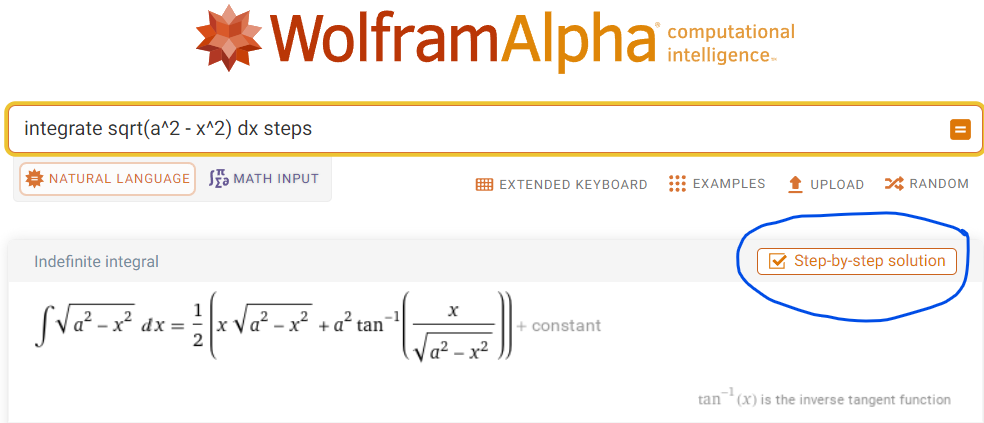
\includegraphics[width=0.9\columnwidth]{graphics/Chap07/WolframAlphaStepByStepSolutions.png}%
    \caption[]{The Wolfram Alpha website provides more information than the Wolfram Plugin for ChatGPT. See the circled box: Step-by-step solution.}
    \label{fig:WolframAlpha}
\end{figure}

\subsection{More on Wolfram Alpha}

Additional features can be accessed through the \href{https://www.wolframalpha.com/examples/pro-features/step-by-step-solutions/step-by-step-calculus}{Wolfram Alpha Website}, such as step-by-step solutions, which are not available through the plugin with ChatGPT. At the present time, the step-by-step solution is a paid feature, with student pricing available. Here is an example of the level of detail provided by Wolfram Alpha's Step-by-Step Solutions feature.

\section*{Indefinite Integral of \( \sqrt{a^2 - x^2} \)}

\textbf{STEP 1} \\
Take the integral:
\[ \int \sqrt{a^2 - x^2} \, dx \]

\textbf{STEP 2} \\
For the integrand \( \sqrt{a^2 - x^2} \), (assuming all variables are positive) substitute \( x = a \sin(u) \) and \( dx = a \cos(u) \, du \). Then \( \sqrt{a^2 - x^2} = \sqrt{a^2 - a^2 \sin^2(u)} = a \cos(u) \) and \( u = \sin^{-1}\left(\frac{x}{a}\right) \):
\[ = a \int a \cos^2(u) \, du \]

\textbf{STEP 3} \\
Factor out constants:
\[ = a^2 \int \cos^2(u) \, du \]

\textbf{STEP 4} \\
Write \( \cos^2(u) \) as \( \frac{1}{2} \cos(2 u) + \frac{1}{2} \):
\[ = a^2 \int \left(\frac{1}{2} \cos(2 u) + \frac{1}{2}\right) \, du \]

\textbf{STEP 5} \\
Integrate the sum term by term and factor out constants:
\[ = \frac{a^2}{2} \int \cos(2 u) \, du + \frac{a^2}{2} \int 1 \, du \]

\textbf{STEP 6} \\
For the integrand \( \cos(2 u) \), substitute \( s = 2 u \) and \( ds = 2 \, du \):
\[ = \frac{a^2}{4} \int \cos(s) \, ds + \frac{a^2}{2} \int 1 \, du \]

\textbf{STEP 7} \\
The integral of \( \cos(s) \) is \( \sin(s) \):
\[ = \frac{a^2}{4} \sin(s) + \frac{a^2}{2} \int 1 \, du \]

\textbf{STEP 8} \\
The integral of 1 is \( u \):
\[ = \frac{a^2}{4} \sin(s) + \frac{a^2 u}{2} + \text{constant} \]

\textbf{STEP 9} \\
Substitute back for \( s = 2 u \):
\[ = \frac{a^2 u}{2} + \frac{a^2}{4} \sin(2 u) + \text{constant} \]

\textbf{STEP 10} \\
Apply the double angle formula \( \sin(2 u) = 2 \sin(u) \cos(u) \):
\[ = \frac{a^2 u}{2} + \frac{a^2}{2} \sin(u) \cos(u) + \text{constant} \]

\textbf{STEP 11} \\
Express \( \cos(u) \) in terms of \( \sin(u) \) using \( \cos^2(u) = 1 - \sin^2(u) \):
\[ = \frac{a^2 u}{2} + \frac{a^2}{2} \sin(u) \sqrt{1 - \sin^2(u)} + \text{constant} \]

\textbf{STEP 12} \\
Substitute back for \( u = \sin^{-1}\left(\frac{x}{a}\right) \):
\[ = \frac{1}{2} x \sqrt{a^2 - x^2} + \frac{a^2}{2} \sin^{-1}\left(\frac{x}{a}\right) + \text{constant} \]

\textbf{STEP 13} \\
Factor the answer a different way:
\[ = \frac{1}{2} \left(x \sqrt{a^2 - x^2} + a^2 \sin^{-1}\left(\frac{x}{a}\right)\right) + \text{constant} \]

\textbf{STEP 14} \\
Which is equivalent for restricted \( x \) and \( a \) values to:
\[ \text{Answer:} \quad \frac{1}{2} \left(x \sqrt{a^2 - x^2} + a^2 \tan^{-1}\left(\frac{x}{\sqrt{a^2 - x^2}}\right)\right) + \text{constant} \]


\section*{Indefinite Integral of \(  x^2 \sin^3(x) \)}

\textbf{STEP 1} \\
Take the integral:
\[ \int x^2 \sin^3(x) \, dx \]

\textbf{STEP 2} \\
For the integrand \( x^2 \sin^3(x) \), use the trigonometric identity \( \sin^2(x) = \frac{1}{2} (1 - \cos(2 x)) \):
\[ = \frac{1}{2} \int x^2 \sin(x) (1 - \cos(2 x)) \, dx \]

\textbf{STEP 3} \\
Expanding the integrand \( x^2 \sin(x) (1 - \cos(2 x)) \) gives \( x^2 \sin(x) - x^2 \sin(x) \cos(2 x) \):
\[ = \frac{1}{2} \int (x^2 \sin(x) - x^2 \sin(x) \cos(2 x)) \, dx \]

\textbf{STEP 4} \\
Integrate the sum term by term and factor out constants:
\[ = -\frac{1}{2} \int x^2 \sin(x) \cos(2 x) \, dx + \frac{1}{2} \int x^2 \sin(x) \, dx \]

\textbf{STEP 5} \\
Use the trigonometric identity \( \sin(\alpha) \cos(\beta) = \frac{1}{2} (\sin(\alpha - \beta) + \sin(\alpha + \beta)) \), where \( \alpha = x \) and \( \beta = 2 x \):
\[ = -\frac{1}{4} \int x^2 (\sin(3 x) - \sin(x)) \, dx + \frac{1}{2} \int x^2 \sin(x) \, dx \]

\textbf{STEP 6} \\
Expanding the integrand \( x^2 (\sin(3 x) - \sin(x)) \) gives \( x^2 \sin(3 x) - x^2 \sin(x) \):
\[ = -\frac{1}{4} \int (x^2 \sin(3 x) - x^2 \sin(x)) \, dx + \frac{1}{2} \int x^2 \sin(x) \, dx \]

\textbf{STEP 7} \\
Integrate the sum term by term and factor out constants:
\[ = -\frac{1}{4} \int x^2 \sin(3 x) \, dx + \frac{3}{4} \int x^2 \sin(x) \, dx \]

\textbf{STEP 8} \\
For the integrand \( x^2 \sin(3 x) \), integrate by parts, \( \int f \, dg = f g - \int g \, df \), where 
\( f = x^2 \), \( dg = \sin(3 x) \, dx \), \( df = 2 x \, dx \), \( g = -\frac{1}{3} \cos(3 x) \):
\[ = \frac{1}{12} x^2 \cos(3 x) - \frac{1}{6} \int x \cos(3 x) \, dx + \frac{3}{4} \int x^2 \sin(x) \, dx \]

\textbf{STEP 9} \\
For the integrand \( x \cos(3 x) \), integrate by parts, \( \int f \, dg = f g - \int g \, df \), where 
\( f = x \), \( dg = \cos(3 x) \, dx \), \( df = dx \), \( g = \frac{1}{3} \sin(3 x) \):
\[ = \frac{1}{12} x^2 \cos(3 x) - \frac{1}{18} x \sin(3 x) + \frac{1}{18} \int \sin(3 x) \, dx + \frac{3}{4} \int x^2 \sin(x) \, dx \]

\textbf{STEP 10} \\
For the integrand \( \sin(3 x) \), substitute \( u = 3 x \) and \( du = 3 dx \):
\[ = \frac{1}{12} x^2 \cos(3 x) - \frac{1}{18} x \sin(3 x) + \frac{1}{54} \int \sin(u) \, du + \frac{3}{4} \int x^2 \sin(x) \, dx \]

\textbf{STEP 11} \\
The integral of \( \sin(u) \) is \( -\cos(u) \):
\[ = -\frac{\cos(u)}{54} + \frac{1}{12} x^2 \cos(3 x) - \frac{1}{18} x \sin(3 x) + \frac{3}{4} \int x^2 \sin(x) \, dx \]

\textbf{STEP 12} \\
For the integrand \( x^2 \sin(x) \), integrate by parts, \( \int f \, dg = f g - \int g \, df \), where 
\( f = x^2 \), \( dg = \sin(x) \, dx \), \( df = 2 x \, dx \), \( g = -\cos(x) \):
\[ = -\frac{\cos(u)}{54} - \frac{3}{4} x^2 \cos(x) + \frac{1}{12} x^2 \cos(3 x) - \frac{1}{18} x \sin(3 x) + \frac{3}{2} \int x \cos(x) \, dx \]

\textbf{STEP 13} \\
For the integrand \( x \cos(x) \), integrate by parts, \( \int f \, dg = f g - \int g \, df \), where 
\( f = x \), \( dg = \cos(x) \, dx \), \( df = dx \), \( g = \sin(x) \):
\[ = -\frac{\cos(u)}{54} - \frac{3}{4} x^2 \cos(x) + \frac{1}{12} x^2 \cos(3 x) + \frac{3}{2} x \sin(x) - \frac{1}{18} x \sin(3 x) - \frac{3}{2} \int \sin(x) \, dx \]

\textbf{STEP 14} \\
The integral of \( \sin(x) \) is \( -\cos(x) \):
\[ = -\frac{\cos(u)}{54} - \frac{3}{4} x^2 \cos(x) + \frac{1}{12} x^2 \cos(3 x) + \frac{3}{2} x \sin(x) - \frac{1}{18} x \sin(3 x) + \frac{3 \cos(x)}{2} + \text{constant} \]

\textbf{STEP 15} \\
Substitute back for \( u = 3 x \):
\[ = -\frac{3}{4} x^2 \cos(x) + \frac{1}{12} x^2 \cos(3 x) + \frac{3}{2} x \sin(x) - \frac{1}{18} x \sin(3 x) + \frac{3 \cos(x)}{2} - \frac{1}{54} \cos(3 x) + \text{constant} \]

\textbf{STEP 16} \\
Which is equal to:
\[ \text{Answer:} \quad \frac{1}{108} (-81 (x^2 - 2) \cos(x) + (9 x^2 - 2) \cos(3 x) - 6 x (\sin(3 x) - 27 \sin(x))) + \text{constant} \]

\



\subsection{UM-GPT: Show me how to Work Example~\ref{ex:aSquaredMinusXsquared} }

The integral $\int \sqrt{a^2 - x^2} \, dx$ can be solved using trigonometric substitution. We will consider the variable $x$ to be $a \sin(\theta)$, where $-\frac{\pi}{2} \leq \theta \leq \frac{\pi}{2}$. This is because $\sin(\theta)$ ranges between -1 and 1, and the expression inside the square root, $a^2 - x^2$, should remain non-negative for real $x$.\\

\textbf{Here is the step-by-step method to evaluate the integral:}

\begin{enumerate}



\item  \textbf{Substitute \(x\) with \(a\sin(\theta)\):}  Let \(x = a\sin(\theta)\). Differentiate this with respect to \(\theta\) to find \(dx\):
\[dx = a\cos(\theta)d\theta\]

\item  \textbf{Express the integral in terms of \(\theta\):} Substitute \(x\) and \(dx\) into the original integral:
\[\int \sqrt{a^2 - (a\sin(\theta))^2} \cdot a\cos(\theta)d\theta\]

\item  \textbf{Simplify the integral:} Simplify the term under the square root and the integral becomes:
\[\int a^2 \cos^2(\theta) d\theta\]

Now, use the double-angle identity for cosine:
\[\cos^2(\theta) = \frac{1 + \cos(2\theta)}{2}\]

The integral now becomes:
\[\int \frac{a^2(1 + \cos(2\theta))}{2} d\theta\]

\item  \textbf{Separate the integral:}  \[\frac{a^2}{2} \int 1 d\theta + \frac{a^2}{2} \int \cos(2\theta) d\theta\]

\item   \textbf{Integrate:} The integration results in:
\[\frac{a^2}{2} \theta + \frac{a^2}{4} \sin(2\theta) + C\]

\item   \textbf{Reverse the trigonometric substitution:}  Recall that \(x = a\sin(\theta)\), so \(\sin(\theta) = \frac{x}{a}\). To find \(\theta\), use the inverse sine function (arcsin):
\[\theta = \arcsin\left(\frac{x}{a}\right)\]

For the term with \(\sin(2\theta)\), use the double-angle identity for sine:
\[\sin(2\theta) = 2\sin(\theta)\cos(\theta)\]

We know that \(\sin(\theta) = \frac{x}{a}\), and since \(\sin^2(\theta) + \cos^2(\theta) = 1\), \(\cos(\theta)\) can be computed by:
\[\cos(\theta) = \sqrt{1 - \sin^2(\theta)} = \sqrt{1 - \left(\frac{x}{a}\right)^2}\]

Hence,
\[\sin(2\theta) = 2\left(\frac{x}{a}\right)\sqrt{1 - \left(\frac{x}{a}\right)^2}\]

\item   \textbf{Plug \(\theta\) and \(\sin(2\theta)\) back into the expression:}

\[\frac{a^2}{2} \arcsin\left(\frac{x}{a}\right) + \frac{a^2}{4} \cdot 2\left(\frac{x}{a}\right)\sqrt{1 - \left(\frac{x}{a}\right)^2} + C\]

\item   \textbf{Simplify:} \[\frac{a^2}{2} \arcsin\left(\frac{x}{a}\right) + \frac{a}{2} x\sqrt{1 - \left(\frac{x}{a}\right)^2} + C\]

\item   \textbf{Write the final answer:} \[\int \sqrt{a^2 - x^2} \, dx = \frac{a^2}{2} \arcsin\left(\frac{x}{a}\right) + \frac{a}{2} x\sqrt{1 - \left(\frac{x}{a}\right)^2} + C\]

\end{enumerate}

This is the final antiderivative of the initial integral in terms of the original variable \(x\).\\


\textcolor{red}{\bf \Large Are you sure the answer is correct for $a < 0$?}\\

My apologies for the oversight. When specifying the domain with respect to the variable \( a \), we need to consider that \( a \) represents the radius of a circle and is typically assumed to be a positive constant in the context of this integral problem. If \( a \) were negative, it would not make sense in terms of the geometry of the circle or the context of the trigonometric substitution we've done (since a radius is always non-negative).

For our integral and the substitutions made, we are working under the assumption that \( a > 0 \). So the answer:

\[
\int \sqrt{a^2 - x^2} \, dx = \frac{a^2}{2} \arcsin\left(\frac{x}{a}\right) + \frac{a}{2} x\sqrt{1 - \left(\frac{x}{a}\right)^2} + C
\]

is correct for the domain of \( x \), assuming \( a > 0 \) and is given by \( -a \leq x \leq a \). This domain corresponds to the values of \( x \) for which the integrand, \( \sqrt{a^2 - x^2} \), is defined and real.

If \( a \) were to be less than zero, we would need to evaluate the integral with the absolute value \( |a| \) instead, to make sure we're working with a positive radius. The final antiderivative would still be correct provided that we interpret \( a \) as \( |a| \) and continue to consider \( x \) within the domain \( -|a| \leq x \leq |a| \), ensuring a non-negative value under the square root. However, the problem is conventionally understood with \( a \) as positive.

\textcolor{blue}{\bf \Large} Can you tell me the domain for which your answer is correct?\\

My apologies for the oversight. When specifying the domain with respect to the variable \( a \), we need to consider that \( a \) represents the radius of a circle and is typically assumed to be a positive constant in the context of this integral problem. If \( a \) were negative, it would not make sense in terms of the geometry of the circle or the context of the trigonometric substitution we've done (since a radius is always non-negative).

For our integral and the substitutions made, we are working under the assumption that \( a > 0 \). So the answer:

\[
\int \sqrt{a^2 - x^2} \, dx = \frac{a^2}{2} \arcsin\left(\frac{x}{a}\right) + \frac{a}{2} x\sqrt{1 - \left(\frac{x}{a}\right)^2} + C
\]

is correct for the domain of \( x \), assuming \( a > 0 \) and is given by \( -a \leq x \leq a \). This domain corresponds to the values of \( x \) for which the integrand, \( \sqrt{a^2 - x^2} \), is defined and real.

If \( a \) were to be less than zero, we would need to evaluate the integral with the absolute value \( |a| \) instead, to make sure we're working with a positive radius. The final antiderivative would still be correct provided that we interpret \( a \) as \( |a| \) and continue to consider \( x \) within the domain \( -|a| \leq x \leq |a| \), ensuring a non-negative value under the square root. However, the problem is conventionally understood with \( a \) as positive.

\section{(Optional Read:) Proofs Associated with the Chapter}

\begin{tcolorbox}[title=\textcolor{black}{Proof of Prop.~\ref{thm:FundamentalTheoremsCalculus} (First Fundamental Theorem of Calculus)}, sharp corners, colback=green!30, colframe=green!80!blue, breakable, fonttitle=\bfseries]

Let \( f:[a, b] \to \real \) be a continuous real-valued function defined on a closed interval \([a, b]\). Then, the function \( F:[a, b] \to \real \) defined by
\begin{equation}
    \label{eq:FirstFundThmCalculusVo1B}
F(x) = \int_a^x f(t) \, dt
\end{equation}
for all \( x \in [a, b]\), is continuous on \([a, b]\), differentiable on the open interval \( (a, b) \), and \( F'(x) = f(x) \) for all \( x \in  (a, b) \). You will also see it written as 
\begin{equation}
    \label{eq:FirstFundThmCalculusVo2B}
   \frac{d}{dx}  F(x) =  \frac{d}{dx} \left[ \int_a^x f(t) \, dt \right] = f(x),
\end{equation}
to emphasize that differentiation undoes, or inverses, integration.
\\

\end{tcolorbox}

\bigskip


\textbf{Proof:} We give a proof that is straightforward and fully rigorous for functions $f:[a, b] \to \real$ that are \textbf{non-decreasing}. The general case is proven in Michigan's Math 451.

\begin{enumerate}[label=\textbf{Claim \arabic*:},leftmargin=*]
    \item \textbf{Continuity of $\bm{F}$:} Because \( f \) is non-decreasing\footnote{If $f(b) \ge 0$, then no absolute value sign is needed on $f(b)$. If $f(b) < 0$, then $f(a) \le f(b) \implies |f(a)| \ge |f(b)| \ge f(b)$. Hence, once again, no absolute value sign is needed.}, 
    $$ M := \max_{x \in [a, b]} |f(x)| = \max \{ |f(a)|, f(b) \} < \infty.$$
Let \( \epsilon > 0 \) and define \( \delta := \frac{\epsilon}{M + 1}>0\). We will show for all \( x, x_0 \in [a, b] \), that \( |x - x_0| < \delta \) implies
$$
|F(x) - F(x_0)| < \epsilon.
$$

\textbf{Proof:} Consider the change in \( F \) as \( x \) varies from \( x_0 \),
$$
F(x) - F(x_0) =  \int_{a}^x f(t) \, dt -  \int_{a}^{x_0} f(t) \, dt = \int_{x_0}^x f(t) \, dt.
$$
This equation holds by the properties of the definite integral, specifically the additivity over adjacent intervals. The absolute value of the integral is bounded by
$$
|F(x) - F(x_0)| = \left| \int_{x_0}^x f(t) \, dt \right| \leq \int_{x_0}^x |f(t)| \, dt.
$$
Given that \( |f(t)| \leq M \) for all \( t \) in \([a, b]\), the integral simplifies further,
$$
|F(x) - F(x_0)| \leq \int_{x_0}^x M \, dt = M |x - x_0|.
$$
The integral \( \int_{x_0}^x M \, dt \) evaluates to \( M \times |x - x_0| \) because the integrand \( M \) is constant, and the length of the interval from \( x_0 \) to \( x \) is \( |x - x_0| \).

Now, by the choice of \( \delta \), if \( |x - x_0| < \delta \) then:
$$
|F(x) - F(x_0)| \leq M |x - x_0| < M \delta = M \left(\frac{\epsilon}{M + 1}\right) < \epsilon.
$$
Thus, we have shown that:
$$
|F(x) - F(x_0)| < \epsilon,
$$
for all \( x \) such that \( |x - x_0| < \delta \). Therefore, \( F \) is continuous at \( x_0 \), and since \( x_0 \) was arbitrary, \( F \) is continuous on \([a, b]\).

    \item \textbf{$ \bm{F'(x) = f(x)}$ for all $\bm{a < x < b}$:}\\
    
   \textbf{Proof:}  Consider the difference quotient for $F$ at some point $x$ in $(a, b)$,
    $$
    \begin{aligned}
        \frac{F(x+h) - F(x)}{h} &= \frac{1}{h} \left( \int_a^{x+h} f(t) \, dt - \int_a^x f(t) \, dt \right) \\
        &=  \frac{1}{h} \int_x^{x+h} f(t) \, dt.
    \end{aligned}
    $$
    Assume first that $h>0$. Then, using once again that $f$ is non-decreasing, 
    $$f(x) \cdot h \le  \int_x^{x+h} f(t) \, dt \le f(x+h) \cdot h.$$
    Plugging into the previous equation and canceling the $h$'s, we have
    $$f(x) \le  \frac{1}{h} \int_x^{x+h} f(t) \, dt \le f(x+h). $$
    Because $f$ is continuous, $\lim_{h \to 0^+} f(x+h) = f(x)$. Therefore, by the Squeeze Theorem, 
    $$ \lim_{h \to 0^+} \frac{1}{h} \int_x^{x+h} f(t) \, dt = f(x).$$
    The same argument can be repeated with minor variations to show that $ \lim_{h \to 0^-} \frac{1}{h} \int_x^{x+h} f(t) \, dt = f(x).$
This completes the proof that $F'(x) = f(x)$, which is a fundamental connection between the differential and integral calculus for continuous functions. 
\end{enumerate}


\Qed


\begin{tcolorbox}[title=\textcolor{black}{Proof of Prop.~\ref{thm:FundamentalTheoremsCalculus} (Second Fundamental Theorem of Calculus)}, sharp corners, colback=green!30, colframe=green!80!blue, breakable, fonttitle=\bfseries]

Let \( f:[a, b] \to \real \) be a real-valued function defined on a closed interval \([a, b]\) that admits an antiderivative \( F \) on \([a, b]\), that is, $F:[a, b] \to \real$ is differentiable on $(a, b)$ and for all $x \in (a, b)$, $F'(x) = f(x)$. Then,  \( f \) is integrable on \([a, b]\) and
\begin{equation}
    \label{eq:SecondFundThmCalculusVo1B}
\int_a^b f(x) \, dx = F(x) \Big|_a^b := F(b) - F(a).
\end{equation}
We rewrite this as 
\begin{equation}
    \label{eq:SecondFundThmCalculusVo2B}
\int_a^b F'(x) \, dx = F(x) \Big|_a^b := F(b) - F(a), 
\end{equation}
to underline that integration undoes, or inverses, differentiation.
\end{tcolorbox}

\bigskip

\textbf{Proof:} We use the method given in \href{https://www2.clarku.edu/faculty/djoyce/ma121/FTCproof.pdf}{Proof of the Fundamental Theorem of Calculus}, Math 121 Calculus II, D Joyce, Spring 2013, with one modification: we ASSUME that $f:[a, b] \to \real$ is continuous, thereby guaranteeing that $f(x) = F'(x)$ is integrable.\\


Define
\[
G(x) = \int_a^x F'(t) \, dt, ~\text{for}~ x \in [a, b].
\]
Then, by the First Fundamental Theorem of Calculus, $G'(x) = F'(x)$. Therefore, $G$ and $F$ differ by a constant $C$, that is, $G(x) - F(x) = C$ for all $x \in [a, b]$. But
\[
G(a) = \int_a^a F'(t) \, dt = 0,
\]
and, therefore,  $G(a) - F(a) = C$, so $\boxed{C = -F(a)}$.\\

It follows that $\boxed{G(x) - F(x) = -F(a)}$ for all $x \in [a, b]$. In particular, $G(b) - F(b) = -F(a)$, so $G(b) = F(b) - F(a)$, that is,
\[
\int_a^b F'(t) \, dt = F(b) - F(a).
\]

This completes the proof that the integral of a function over an interval is equal to the difference in the values of any of its antiderivatives evaluated at the endpoints of the interval, affirming that integration can be seen as the inverse operation to differentiation.

\Qed

\bigskip 
\emstat{
\begin{center}
    
\bf \large We next explore how restrictive it was to assume that a function is non-decreasing. 
\end{center}
}

\bigskip



\textbf{1) Property of max and min functions:} For any \( y \in \mathbb{R} \), the functions \(\max(y,0)\) and \(\min(y,0)\) have the property that:
\[
\max(y, 0) + \min(y, 0) = y
\]

\textit{Proof:} Consider two cases based on the value of \( y \):

\textbf{Case 1:} \( y \geq 0 \). In this case, we have
\[
\max(y, 0) = y \quad \text{and} \quad \min(y, 0) = 0
\]
Thus,
\[
\max(y, 0) + \min(y, 0) = y + 0 = y
\]

\textbf{Case 2:} \( y < 0 \). In this case, we have
\[
\max(y, 0) = 0 \quad \text{and} \quad \min(y, 0) = y
\]
Thus,
\[
\max(y, 0) + \min(y, 0) = 0 + y = y
\]

In both cases, \(\max(y, 0) + \min(y, 0)\) simplifies to \( y \), proving the statement.
\Qed

\bigskip

\textbf{2) Decomposition of continuously differentiable functions:}  If \( f: [a, b] \to \mathbb{R} \) is a continuously differentiable function, then \( f \) can be expressed as the difference of two continuous, non-decreasing functions. \\

\textit{Construction:} Define two functions \( g \) and \( k \) over \([a, b]\) by:
\[
g(x) = f(a) + \int_a^x \max(f'(t), 0) \, dt 
\]
and
\[
k(x) = -\int_a^x \min(f'(t), 0) \, dt
\]

\textit{Properties:}  Since \( f \) is continuously differentiable, \( f' \) exists and is continuous. The function \( g \) is non-decreasing because the integrand, \(\max(f'(t), 0)\), is non-negative and strictly positive whenever \( f'(t) > 0 \). \\

The function \( k \) is non-decreasing because the integrand \(-\min(f'(t), 0)\) is non-negative, being zero when \( f'(t) \geq 0 \) and positive when \( f'(t) < 0 \).\\

\textit{Expressing \( f \) as a difference:}
\begin{align*}
g(x) - k(x) &=  f(a) + \left( \int_a^x \max(f'(t), 0) \, dt \right) - \left( -\int_a^x \min(f'(t), 0) \, dt \right) \\
&= f(a) +  \int_a^x (\max(f'(t), 0) + \min(f'(t), 0)) \, dt  \\
&= f(a) +  \int_a^x f'(t) \, dt  \\
&= f(a) + \left(f(x) - f(a)\right) \\
&= f(x).
\end{align*}

\bigskip

This construction expresses \( f \) as the difference of two continuous, non-decreasing functions over the interval \([a, b]\). Hence, the proof of Prop.~\ref{thm:FundamentalTheoremsCalculus} given for non-decreasing functions can be applied to functions that are continuously differentiable.


